% Options for packages loaded elsewhere
% Options for packages loaded elsewhere
\PassOptionsToPackage{unicode}{hyperref}
\PassOptionsToPackage{hyphens}{url}
\PassOptionsToPackage{dvipsnames,svgnames,x11names}{xcolor}
%
\documentclass[
  spanish,
  letterpaper,
]{scrreprt}
\usepackage{xcolor}
\usepackage{amsmath,amssymb}
\setcounter{secnumdepth}{5}
\usepackage{iftex}
\ifPDFTeX
  \usepackage[T1]{fontenc}
  \usepackage[utf8]{inputenc}
  \usepackage{textcomp} % provide euro and other symbols
\else % if luatex or xetex
  \usepackage{unicode-math} % this also loads fontspec
  \defaultfontfeatures{Scale=MatchLowercase}
  \defaultfontfeatures[\rmfamily]{Ligatures=TeX,Scale=1}
\fi
\usepackage{lmodern}
\ifPDFTeX\else
  % xetex/luatex font selection
\fi
% Use upquote if available, for straight quotes in verbatim environments
\IfFileExists{upquote.sty}{\usepackage{upquote}}{}
\IfFileExists{microtype.sty}{% use microtype if available
  \usepackage[]{microtype}
  \UseMicrotypeSet[protrusion]{basicmath} % disable protrusion for tt fonts
}{}
\makeatletter
\@ifundefined{KOMAClassName}{% if non-KOMA class
  \IfFileExists{parskip.sty}{%
    \usepackage{parskip}
  }{% else
    \setlength{\parindent}{0pt}
    \setlength{\parskip}{6pt plus 2pt minus 1pt}}
}{% if KOMA class
  \KOMAoptions{parskip=half}}
\makeatother
% Make \paragraph and \subparagraph free-standing
\makeatletter
\ifx\paragraph\undefined\else
  \let\oldparagraph\paragraph
  \renewcommand{\paragraph}{
    \@ifstar
      \xxxParagraphStar
      \xxxParagraphNoStar
  }
  \newcommand{\xxxParagraphStar}[1]{\oldparagraph*{#1}\mbox{}}
  \newcommand{\xxxParagraphNoStar}[1]{\oldparagraph{#1}\mbox{}}
\fi
\ifx\subparagraph\undefined\else
  \let\oldsubparagraph\subparagraph
  \renewcommand{\subparagraph}{
    \@ifstar
      \xxxSubParagraphStar
      \xxxSubParagraphNoStar
  }
  \newcommand{\xxxSubParagraphStar}[1]{\oldsubparagraph*{#1}\mbox{}}
  \newcommand{\xxxSubParagraphNoStar}[1]{\oldsubparagraph{#1}\mbox{}}
\fi
\makeatother


\usepackage{longtable,booktabs,array}
\newcounter{none} % for unnumbered tables
\usepackage{calc} % for calculating minipage widths
% Correct order of tables after \paragraph or \subparagraph
\usepackage{etoolbox}
\makeatletter
\patchcmd\longtable{\par}{\if@noskipsec\mbox{}\fi\par}{}{}
\makeatother
% Allow footnotes in longtable head/foot
\IfFileExists{footnotehyper.sty}{\usepackage{footnotehyper}}{\usepackage{footnote}}
\makesavenoteenv{longtable}
\usepackage{graphicx}
\makeatletter
\newsavebox\pandoc@box
\newcommand*\pandocbounded[1]{% scales image to fit in text height/width
  \sbox\pandoc@box{#1}%
  \Gscale@div\@tempa{\textheight}{\dimexpr\ht\pandoc@box+\dp\pandoc@box\relax}%
  \Gscale@div\@tempb{\linewidth}{\wd\pandoc@box}%
  \ifdim\@tempb\p@<\@tempa\p@\let\@tempa\@tempb\fi% select the smaller of both
  \ifdim\@tempa\p@<\p@\scalebox{\@tempa}{\usebox\pandoc@box}%
  \else\usebox{\pandoc@box}%
  \fi%
}
% Set default figure placement to htbp
\def\fps@figure{htbp}
\makeatother

\ifLuaTeX
  \usepackage{luacolor}
  \usepackage[soul]{lua-ul}
\else
  \usepackage{soul}
\fi

% definitions for citeproc citations
\NewDocumentCommand\citeproctext{}{}
\NewDocumentCommand\citeproc{mm}{%
  \begingroup\def\citeproctext{#2}\cite{#1}\endgroup}
\makeatletter
 % allow citations to break across lines
 \let\@cite@ofmt\@firstofone
 % avoid brackets around text for \cite:
 \def\@biblabel#1{}
 \def\@cite#1#2{{#1\if@tempswa , #2\fi}}
\makeatother
\newlength{\cslhangindent}
\setlength{\cslhangindent}{1.5em}
\newlength{\csllabelwidth}
\setlength{\csllabelwidth}{3em}
\newenvironment{CSLReferences}[2] % #1 hanging-indent, #2 entry-spacing
 {\begin{list}{}{%
  \setlength{\itemindent}{0pt}
  \setlength{\leftmargin}{0pt}
  \setlength{\parsep}{0pt}
  % turn on hanging indent if param 1 is 1
  \ifodd #1
   \setlength{\leftmargin}{\cslhangindent}
   \setlength{\itemindent}{-1\cslhangindent}
  \fi
  % set entry spacing
  \setlength{\itemsep}{#2\baselineskip}}}
 {\end{list}}
\usepackage{calc}
\newcommand{\CSLBlock}[1]{\hfill\break\parbox[t]{\linewidth}{\strut\ignorespaces#1\strut}}
\newcommand{\CSLLeftMargin}[1]{\parbox[t]{\csllabelwidth}{\strut#1\strut}}
\newcommand{\CSLRightInline}[1]{\parbox[t]{\linewidth - \csllabelwidth}{\strut#1\strut}}
\newcommand{\CSLIndent}[1]{\hspace{\cslhangindent}#1}

\ifLuaTeX
\usepackage[bidi=basic,shorthands=off]{babel}
\else
\usepackage[bidi=default,shorthands=off]{babel}
\fi
\ifLuaTeX
  \usepackage{selnolig} % disable illegal ligatures
\fi


\setlength{\emergencystretch}{3em} % prevent overfull lines

\providecommand{\tightlist}{%
  \setlength{\itemsep}{0pt}\setlength{\parskip}{0pt}}



 


\usepackage{tikz}
\usetikzlibrary{arrows.meta, positioning, calc}
\makeatletter
\@ifpackageloaded{tcolorbox}{}{\usepackage[skins,breakable]{tcolorbox}}
\@ifpackageloaded{fontawesome5}{}{\usepackage{fontawesome5}}
\definecolor{quarto-callout-color}{HTML}{909090}
\definecolor{quarto-callout-note-color}{HTML}{0758E5}
\definecolor{quarto-callout-important-color}{HTML}{CC1914}
\definecolor{quarto-callout-warning-color}{HTML}{EB9113}
\definecolor{quarto-callout-tip-color}{HTML}{00A047}
\definecolor{quarto-callout-caution-color}{HTML}{FC5300}
\definecolor{quarto-callout-color-frame}{HTML}{acacac}
\definecolor{quarto-callout-note-color-frame}{HTML}{4582ec}
\definecolor{quarto-callout-important-color-frame}{HTML}{d9534f}
\definecolor{quarto-callout-warning-color-frame}{HTML}{f0ad4e}
\definecolor{quarto-callout-tip-color-frame}{HTML}{02b875}
\definecolor{quarto-callout-caution-color-frame}{HTML}{fd7e14}
\makeatother
\makeatletter
\@ifpackageloaded{bookmark}{}{\usepackage{bookmark}}
\makeatother
\makeatletter
\@ifpackageloaded{caption}{}{\usepackage{caption}}
\AtBeginDocument{%
\ifdefined\contentsname
  \renewcommand*\contentsname{Tabla de contenidos}
\else
  \newcommand\contentsname{Tabla de contenidos}
\fi
\ifdefined\listfigurename
  \renewcommand*\listfigurename{Listado de Figuras}
\else
  \newcommand\listfigurename{Listado de Figuras}
\fi
\ifdefined\listtablename
  \renewcommand*\listtablename{Listado de Tablas}
\else
  \newcommand\listtablename{Listado de Tablas}
\fi
\ifdefined\figurename
  \renewcommand*\figurename{Figura}
\else
  \newcommand\figurename{Figura}
\fi
\ifdefined\tablename
  \renewcommand*\tablename{Tabla}
\else
  \newcommand\tablename{Tabla}
\fi
}
\@ifpackageloaded{float}{}{\usepackage{float}}
\floatstyle{ruled}
\@ifundefined{c@chapter}{\newfloat{codelisting}{h}{lop}}{\newfloat{codelisting}{h}{lop}[chapter]}
\floatname{codelisting}{Listado}
\newcommand*\listoflistings{\listof{codelisting}{Listado de Listados}}
\usepackage{amsthm}
\theoremstyle{definition}
\newtheorem{definition}{Definición}[chapter]
\theoremstyle{remark}
\AtBeginDocument{\renewcommand*{\proofname}{Demostración}}
\newtheorem*{remark}{Observación}
\newtheorem*{solution}{Solución}
\newtheorem{refremark}{Observación}[chapter]
\newtheorem{refsolution}{Solución}[chapter]
\makeatother
\makeatletter
\makeatother
\makeatletter
\@ifpackageloaded{caption}{}{\usepackage{caption}}
\@ifpackageloaded{subcaption}{}{\usepackage{subcaption}}
\makeatother
\usepackage{bookmark}
\IfFileExists{xurl.sty}{\usepackage{xurl}}{} % add URL line breaks if available
\urlstyle{same}
\hypersetup{
  pdftitle={Fitted Q-Iteration: Estimación de niveles de presas},
  pdfauthor={Erika Rubí Jiménez Guzmán; Asesor: Dr.~Yofre Hernán García Gómez},
  pdflang={es},
  colorlinks=true,
  linkcolor={blue},
  filecolor={Maroon},
  citecolor={Blue},
  urlcolor={Blue},
  pdfcreator={LaTeX via pandoc}}


\title{Fitted Q-Iteration: Estimación de niveles de presas}
\author{Erika Rubí Jiménez Guzmán \and Asesor: Dr.~Yofre Hernán García
Gómez}
\date{2026-11-13}
\begin{document}
\begin{titlepage}
\hspace{-1.7cm} %Este comando es para mandar a la izquierda ;)
%Aquí empiezan los tres minipages de antes
\begin{minipage}[t][0.03\textheight][c]{0.22\textwidth}
        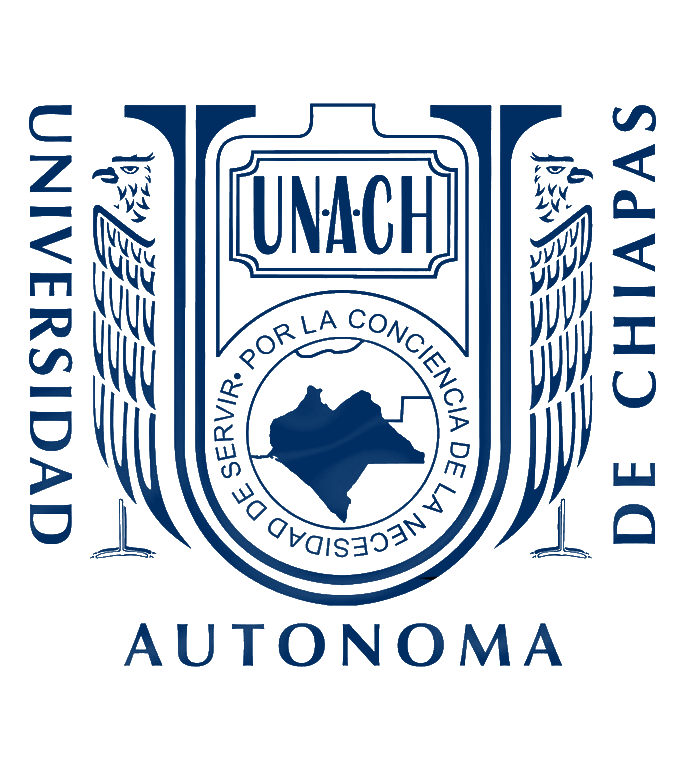
\includegraphics[width=3.7cm]{Imagenes/logo-unach.png}
\end{minipage}\hspace{0.9cm}
\begin{minipage}[t][0.03\textheight][c]{0.69\textwidth}
\begin{center}
                \textsc{\huge Universidad Autónoma de Chiapas}\\[0.3cm]
                \hrule height 2.5pt
                \vspace{0.2cm}
                \hrule height1pt
                \vspace{0.5cm}
                \textsc{\Large Facultad de Ciencias en Física y Matemáticas}
\end{center}
\end{minipage}\hspace{0.2cm}
\begin{minipage}[t][0.03\textheight][c]{0.2\textwidth}
		
\includegraphics[width=2.7cm]{Imagenes/FCFMLOGO.png}
\end{minipage}\\
%%%%%%%%%%%%%%%%%%Aquí comienzan los otros dos minipages del título%%%%%%%%%%%%%%%%%%%%%%%%%%%%%%%%%%%%%%%%%%%%%%%%%%%%%%%%%%%%%%%%%%%%%%%%%%%%%%%%%%%%%%%%%%%%%%
\begin{minipage}[t][0.93\textheight][c]{0.06\textwidth}
\vspace{65pt}
    \vspace{5cm}
    \begin{center}
        \vrule width1pt height18cm
        \vspace{5mm}
        \vrule width2.5pt height18cm
        \vspace{5mm}
        \vrule width1pt height18cm
   \end{center}
\end{minipage}\hspace{1.3cm} %Esto mueve las letras que tienes ahí
\begin{minipage}[t][0.95\textheight][c]{0.76\textwidth}
            \vspace{5cm}
            \begin{center}
                {\Large\bfseries Fitted Q-Iteration: Estimación de niveles de presas}\\[2cm]
                \textsc{\huge \textbf{T\, E\, S\, I\, S}}\\[1.5cm]
                \textsc{\large QUE PARA OBTENER EL TÍTULO DE:}\\[0.3cm]
                \textbf{\textsc{LICENCIADA EN MATEMÁTICAS APLICADAS}}\\[1.5cm]
                \textsc{\large PRESENTA:}\\[0.3cm]
                \textbf{\textsc{\large {ERIKA RUBÍ JIMÉNEZ GUZMÁN}}}\\[2cm]
                {\large\scshape Director:\\[0.3cm]
                {\textbf{\large Dr. Yofre Hernán García Gómez }}}\\[2.0cm]
                \large{Tuxtla Gutiérrez, Chiapas a \today.}

            \end{center}
\end{minipage}
\end{titlepage}

\pagebreak[2]

\chapter*{Dedicatoria}
\begin{flushright}
\textit{A mis padres y hermanos, \\ por su apoyo incondicional y absoluta fe en mí. Esta tesis es mi manera de agradecerles su amor, paciencia y sacrificio.}
\end{flushright}

\chapter*{Agradecimientos}
En primer lugar, deseo agradecer de todo corazón a mi director de tesis, el Dr. Yofre Hernán García Gómez. Gracias por su apoyo y fe, no solo en el presente trabajo sino también en mí. El tiempo que ha invertido en mi persona ha sido un regalo de lo más valioso; gracias a su guía y mentoría he logrado adquirir conocimientos que nunca habría imaginado alcanzar por mi cuenta. Esta tesis es el fruto directo de su apoyo como tutor y de la colaboración entre la escuela de matemáticas y la de física, por lo que estoy profundamente agradecido.

Asimismo, quiero expresar mi profundo agradecimiento a mis estimados profesores y profesoras, pues todos y cada uno de ellos aportaron a mi formación académica con pasión y dedicación genuinas, a veces yendo más allá del deber para explicar un tema o un ejercicio con tal de transmitir su vasto conocimiento. Además, quiero agradecer al personal administrativo y de la biblioteca, quienes, además de desempeñar con excelencia su labor, me brindaron su amistad; eso fue un maravilloso regalo que atesoraré en mi corazón.

Adicionalmente, mi gratitud se extiende a mis maravillosos y amados amigos Wilson, Noé, Tass, Wicho, Kevin, Yahir, Lalo y Javier. Gracias por su apoyo incondicional ante todas las adversidades y problemas; su presencia fue fundamental en esta etapa de mi vida. Agradezco cada risa, momento, conversación y hasta discusión compartida con ustedes. Todos y cada uno me inspiraron, alentaron y enseñaron a crecer no solo como estudiante, sino como persona; me mostraron su determinación y voluntad para no rendirse, pero también que está bien tomar un descanso y compartir aquello que nos aqueja con nuestros seres queridos. Son verdaderamente los mejores amigos que pude desear y su contribución a este logro es imposible de omitir.

Por último, pero no menos importante, expreso mi profundo agradecimiento a mis padres, Zoila y Eczar; y a mis hermanos, Eczar y María. Su amor y apoyo incondicionales me han llevado hasta aquí, a una meta que creí tan lejos y que hoy veo realizada. Son incontables los sacrificios que han realizado en pro de mi bienestar, tanto físico como mental, cargando con pesos que en cierto momento me resultaban imposibles de sobrellevar. No tengo palabras para describir la gratitud que siento hacia ustedes; siempre estaré orgulloso de ser llamado su hijo y su hermano. Los amo con todo mi corazón.

A todos ustedes, mi más sincero agradecimiento. Este logro no habría sido posible sin su apoyo, generosidad y aliento constante.
\renewcommand*\contentsname{Tabla de contenidos}
{
\setcounter{tocdepth}{2}
\tableofcontents
}

\bookmarksetup{startatroot}

\chapter*{Resumen}\label{resumen}
\addcontentsline{toc}{chapter}{Resumen}

\markboth{Resumen}{Resumen}

Aquí pondré un resumen de mi tesis, que se llama ``Fitted Q-Iteration:
Estimación de niveles de presas''.

\bookmarksetup{startatroot}

\chapter*{Introduction}\label{introduction}
\addcontentsline{toc}{chapter}{Introduction}

\markboth{Introduction}{Introduction}

Esta será la introducción.

ejemplo de una cita Puterman (\citeproc{ref-puterman1994markov}{1994}).

\part{Preliminares}

\chapter{Fundamentos Matemáticos}\label{fundamentos-matemuxe1ticos}

\section{Inteligencia Artificial (IA)}\label{inteligencia-artificial-ia}

La \textbf{Inteligencia Artificial (IA)} es un campo de estudio que se
centra en la creación de sistemas capaces de realizar tareas que
normalmente requieren inteligencia humana. La IA combina diversas
disciplinas, incluyendo matemáticas, estadísticas, informática y
neurociencia, para desarrollar algoritmos y modelos que permiten a las
máquinas aprender, razonar y tomar decisiones de manera autónoma.

Este campo está dividido en varias subáreas, cada una con su enfoque y
aplicaciones específicas. Entre las más destacadas se encuentran el
\textbf{Aprendizaje Automático (Machine Learning)}, \textbf{Aprendizaje
Profundo (Deep Learning)}, \textbf{Procesamiento del Lenguaje Natural},
\textbf{Visión por Computadora}, \textbf{Robótica}, entre otras. Cada
una de estas subáreas utiliza diferentes técnicas y enfoques para
abordar problemas complejos y mejorar la capacidad de las máquinas para
interactuar con el mundo que las rodea.

\subsection{Aprendizaje Automático}\label{aprendizaje-automuxe1tico}

En este subcampo de la Inteligencia Artificial, las máquinas aprenden a
partir de datos, similar a como lo hacemos nosotros, permitiendoles
mejorar con la experiencia. El aprendizaje automático se basa en
algoritmos que identifican patrones y relaciones en los datos, lo que
permite a las máquinas hacer predicciones o tomar decisiones sin ser
explícitamente programadas para cada tarea específica. Este enfoque ha
revolucionado diversas industrias, desde la medicina hasta la economía,
al proporcionar herramientas más eficientes y precisas para el análisis
de datos y la toma de decisiones.

El aprendizaje automático se clasifica en tres categorías principales:
\textbf{Aprendizaje Supervisado}, \textbf{Aprendizaje No Supervisado} y
\textbf{Aprendizaje por Refuerzo}, cada una con sus propias técnicas y
aplicaciones. Estas categorías permiten abordar diferentes tipos de
problemas y desafíos, desde la clasificación de datos hasta la
optimización de estrategias en entornos dinámicos.

\begin{definition}[Aprendizaje
Supervisado]\protect\hypertarget{def-sub}{}\label{def-sub}

Esta categoría se basa en utilizar conjuntos de datos etiquetados (datos
de entrada con sus correspondientes salidas) para entrenar modelos
matemáticos que puedan identificar patrones y a partir de ellos predecir
resultados futuros sobre datos nuevos.

Este tipo de aprendizaje es principalmente utilizado en:

\begin{itemize}
\tightlist
\item
  \textbf{\emph{Tareas de clasificación:}} los modelos predicen la clase
  a las que pertenece cada dato. Por ejemplo, identificar si un correo
  electrónico es spam o no.
\item
  \textbf{\emph{Regresión:}} predicen valores numéricos a partir de
  datos de entrada. Por ejemplo, predecir el precio de una vivienda
  basado en sus características.
\end{itemize}

\end{definition}

\begin{definition}[Aprendizaje No
Supervisado]\protect\hypertarget{def-sub}{}\label{def-sub}

A diferencia del aprendizaje supervisado, en este tipo de aprendizaje no
se utilizan datos etiquetados. En su lugar, los algoritmos buscan
patrones ocultos o agrupaciones dentro de los datos. Estos modelos son
utilizados para tareas especificas como:

\begin{itemize}
\tightlist
\item
  \textbf{\emph{Agrupamiento (Clustering):}} los modelos identifican
  grupos de datos similares entre sí. Por ejemplo, segmentar clientes en
  diferentes grupos según sus comportamientos de compra.
\item
  \textbf{\emph{Reducción de dimensionalidad:}} los modelos simplifican
  los datos manteniendo la mayor cantidad de información posible. Por
  ejemplo, reducir el número de variables en un conjunto de datos para
  facilitar su análisis.
\end{itemize}

\end{definition}

\begin{definition}[Aprendizaje por
Refuerzo]\protect\hypertarget{def-sub}{}\label{def-sub}

En este tipo de aprendizaje automático, los agentes autónomos aprenden a
tomar decisiones a partir de la interección con un entorno en el cual
reciben recompensas o penalizaciones según sus acciones. A continuación
se presentan los conceptos fundamentales de este tipo de aprendizaje

\begin{itemize}
\item
  \textbf{\emph{Agente:}} es el decisor, este selecciona las acciones en
  cada estado.
\item
  \textbf{\emph{Entorno:}} descrito como un Markov Decision Process
  (MDP), el entorno se define como
  \((\mathcal{S}, \mathcal{A}, \mathbb{P}, \mathcal{R})\), en donde

  \begin{itemize}
  \tightlist
  \item
    \(\mathcal{S}\) es el conjunto de estados,
  \item
    \(\mathcal{A}\) es el conjunto de acciones,
  \item
    \(\mathbb{P}\) es la función de transición de probabilidad,\\
  \item
    \(\mathcal{R}\) es la función de recompensa.
  \end{itemize}
\item
  \textbf{\emph{Estado}} \((\mathcal{S})\): situación actual del agente
  en el entorno.
\item
  \textbf{\emph{Acción}} \((\mathcal{A})\): decisión elegida por agente
  en el estado \(s \in \mathcal{S}\). El conjunto de acciones posibles
  en un estado se denota como \(\mathcal{A}(s)\).
\item
  \textbf{\emph{Recompensa}} \((\mathcal{R})\): función que asigna un
  valor numérico a cada par \((s, a)\), indicando el beneficio o costo
  de esa acción.
\item
  \textbf{\emph{Política}} \((\pi)\): regla de decisión que especifica
  cómo el agente selecciona acciones en cada estado. La política puede
  ser:

  \begin{itemize}
  \tightlist
  \item
    Determinista \(\pi(s) = a\): dado un estado \(s\), el agente
    selecciona una única acción \(a\).
  \item
    Estocástica \(\pi(a|s) = P(A_t = a | S_t = s)\): asigna una
    probabilidad a cada acción \(a\) posible en un estado determinado
    \(s\).
  \end{itemize}
\end{itemize}

El aprendizaje por refuerzo se centra esencialmente en la relación entre
un agente, entorno y el objetivo (lo que se desea lograr). La literatura
formula esta relación en términos de un \textbf{Proceso de Decisión de
Markov (MDP)}.

\begin{figure}

\centering{

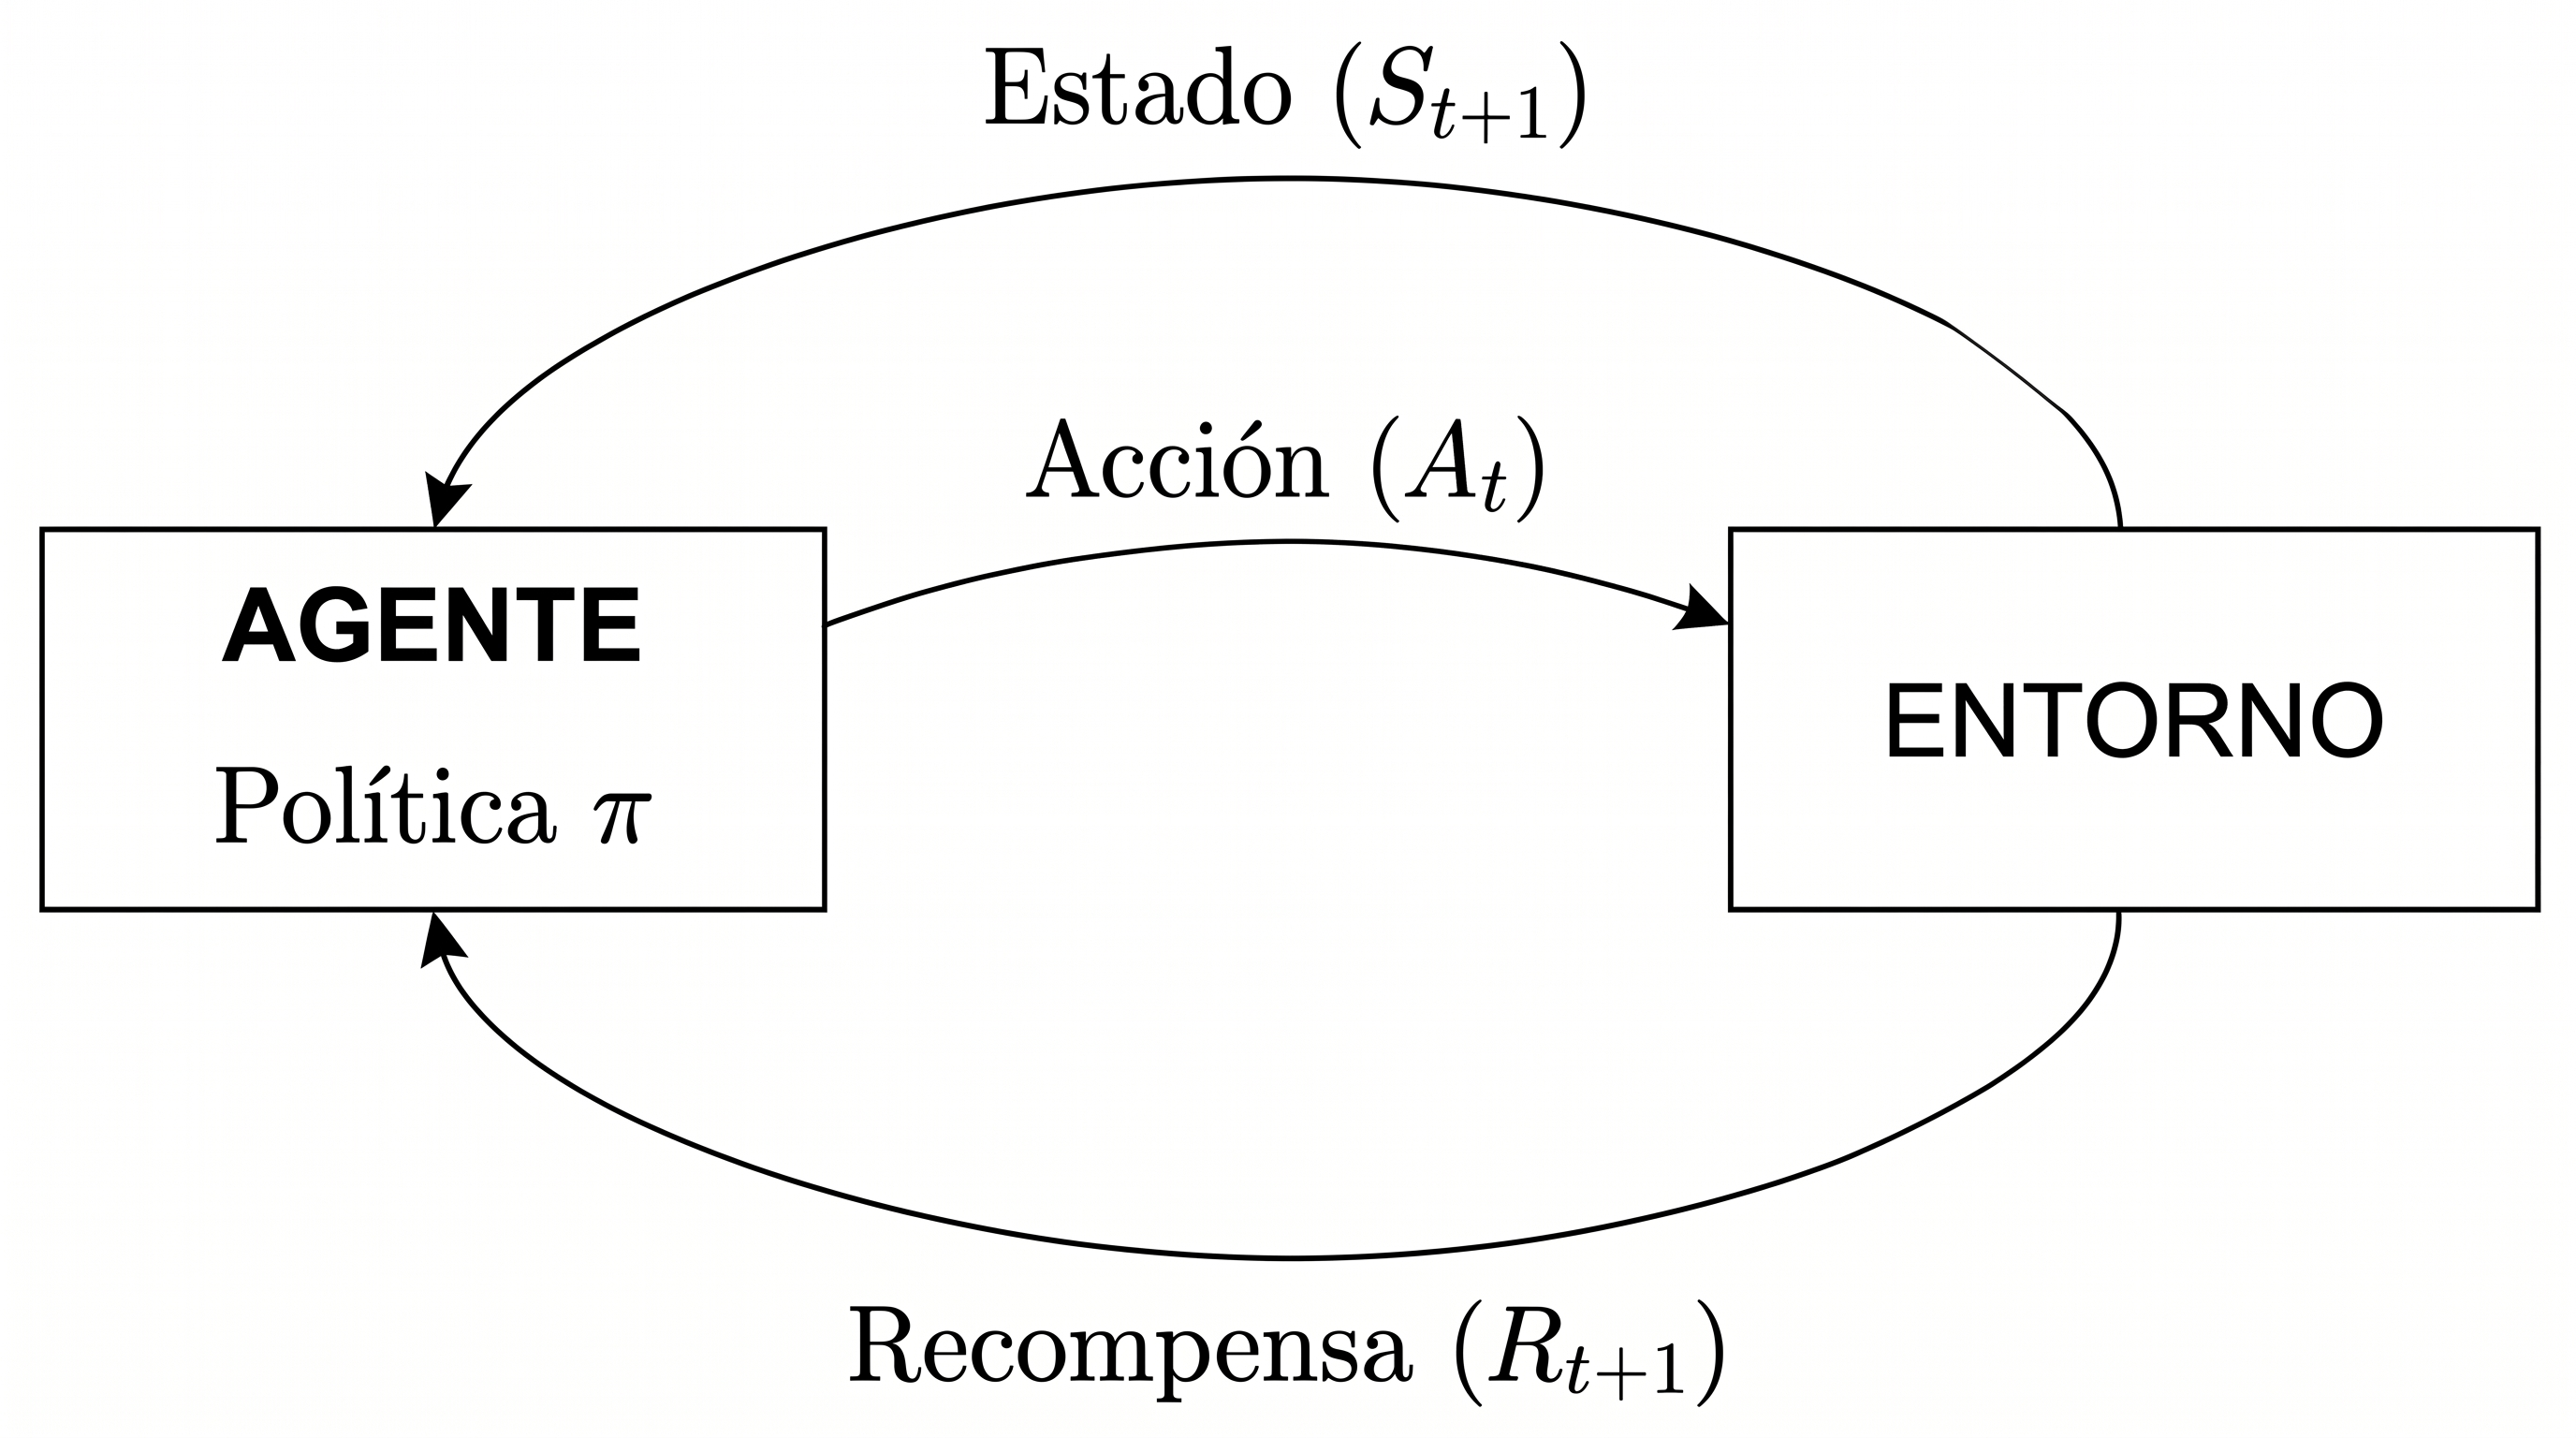
\includegraphics[width=1\linewidth,height=\textheight,keepaspectratio]{Imagenes/diagramaRL.jpg}

}

\caption{\label{fig-diagramaRL}Diagrama del proceso de interacción en el
aprendizaje por refuerzo.}

\end{figure}%

\end{definition}

Véase IBM (\citeproc{ref-ibmRL}{2025}) para más información sobre estos
tipos de aprendizaje y sus aplicaciones.

\subsubsection{Q-Learning}\label{q-learning}

Existen distintos algoritmos de aprendizaje por refuerzo, entre los
cuales se encuentra el \textbf{Q-Learning}, este permite a un agente
aprender a tomar decisiones en un entorno para maximizar una recompensa
acumulada a lo largo del tiempo. Este modelo es model-free, es decir, no
requiere un modelo del entorno para aprender, sino que se basa en la
experiencia directa del agente a través de la exploración y explotación
de su entorno.

\chapter{Fundamentos del Sistema
Hidroeléctrico}\label{fundamentos-del-sistema-hidroeluxe9ctrico}

\section{Configuración Hidrológica y Operativa de la Cuenca del Río
Grijalva}\label{configuraciuxf3n-hidroluxf3gica-y-operativa-de-la-cuenca-del-ruxedo-grijalva}

El sistema hidroeléctrico del río Grijalva, localizado en el sureste de
México entre los estados de Chiapas y Tabasco, representa la
infraestructura hidroenergética más importante del país, aportando una
fracción sustancial de la energía hidroeléctrica del Sistema Eléctrico
Nacional. El complejo hidrológico comprende cuatro grandes centrales
hidroeléctricas dispuestas en serie a lo largo del cauce principal del
río: La Angostura (Belisario Domínguez), Chicoasén (Manuel Moreno
Torres), Malpaso (Nezahualcóyotl) y Peñitas (Ángel Albino Corzo).

Desde una perspectiva operativa e hidrológica, los cuatro embalses
presentan marcadas diferencias estructurales en sus capacidades de
almacenamiento útil: - \textbf{La Angostura:} Es el embalse de cabecera
con la mayor capacidad de almacenamiento del país
(\(16,200\text{ hm}^3\) en su nivel de aguas máximas ordinarias),
funcionando como el principal vaso regulador plurianual de la cuenca
alta. - \textbf{Chicoasén:} Es una central hidroeléctrica de muy alta
caída hidráulica con un vaso de regulación pequeña, cuya dinámica
operativa consiste fundamentalmente en turbinar el agua descargada por
La Angostura, operando a nivel de vaso prácticamente constante. -
\textbf{Malpaso:} Es el segundo gran embalse del sistema
(\(9,600\text{ hm}^3\) de capacidad máxima), ubicado en la cuenca media.
Recibe directamente los volúmenes turbinados y derramados por La
Angostura y Chicoasén, más las aportaciones tributarias de su cuenca
propia intermedia. - \textbf{Peñitas:} Es la obra de toma y regulación
terminal de la cascada, con capacidad de almacenamiento reducida, cuya
misión primordial es amortiguar las fluctuaciones horarias de turbinado
y regular el gasto hacia la planicie de Tabasco.

Conforme a la metodología establecida por Díaz
(\citeproc{ref-Alegria2010}{2010}), esta asimetría estructural justifica
plenamente modelar la cascada a través de un \textbf{sistema equivalente
de dos presas mayores con acoplamiento hidráulico en serie}: 1. El
subsistema superior, constituido por la presa \textbf{La Angostura}, la
cual incorpora en su beneficio de generación la carga hidráulica
efectiva aportada aguas abajo por la presa \textbf{Chicoasén}. 2. El
subsistema inferior, integrado por la presa \textbf{Malpaso}, que recibe
en tránsito los caudales desfogados por el subsistema superior,
incorpora las afluencias por cuenca propia intermedia y absorbe en su
salto hidráulico el beneficio de la presa \textbf{Peñitas}.

\section{El Problema de Optimización Operativa
Multiobjetivo}\label{el-problema-de-optimizaciuxf3n-operativa-multiobjetivo}

La gestión operativa del sistema del río Grijalva involucra un conflicto
estructural entre dos entidades gubernamentales con objetivos
contrapuestos (Díaz (\citeproc{ref-Alegria2010}{2010})): 1.
\textbf{Comisión Federal de Electricidad (CFE):} Cuyo mandato rector es
maximizar la generación de energía eléctrica limpia y firme, lo que
incentiva mantener los embalses en cotas elevadas para maximizar la
carga neta disponible en las turbinas hidroeléctricas. 2.
\textbf{Comisión Nacional del Agua (CONAGUA):} Cuyo mandato
institucional es mitigar los riesgos de inundación en las poblaciones
ribereñas y centros urbanos de la planicie tabasqueña (especialmente
Villahermosa), lo que exige mantener un volumen de resguardo o capacidad
de amortiguamiento libre ante crecidas extraordinarias durante la
temporada ciclónica.

Para conciliar estos requerimientos, el Comité Técnico de Operación de
Obras Hidráulicas (CTOOH) establece una \textbf{curva guía} (o curva
índice estacional de seguridad), la cual define la trayectoria máxima de
almacenamiento admisible a lo largo del año. La optimización de la
operación consiste en determinar la regla de extracción de agua de cada
vaso que maximice la energía esperada, garantice la confiabilidad de
suministro (evitando déficits en estiaje) y minimice estrictamente los
vertidos incontrolados y las violaciones a la curva guía.

\begin{definition}[Fitted
Q-Iteration]\protect\hypertarget{def-sub}{}\label{def-sub}

Algoritmo Offline (aprende analizando el historial de
experiencias)\ldots{}

\end{definition}

\part{Modelo Matemático}

\chapter{Modelo Matemático de Programación Dinámica Estocástica para
Optimizar la Operación de un Sistema
Hidroeléctrico}\label{modelo-matemuxe1tico-de-programaciuxf3n-dinuxe1mica-estocuxe1stica-para-optimizar-la-operaciuxf3n-de-un-sistema-hidroeluxe9ctrico}

En este capítulo se presenta una formulación rigurosa del problema de
optimización de la operación de un sistema hidroeléctrico mediante un
Proceso de Decisión de Markov (MDP), usando Programación Dinámica
Estocástica (PDE) con el fin de obtener la política óptima de operación
tomando en cuenta el concepto de curva guía. Se trata de un método
exacto: la función de valor se almacena como una tabla indexada por los
estados discretizados del sistema y se calcula mediante retropropagación
de Bellman (\emph{Backward Induction}).

Lo anterior se propone tal y como lo describe Díaz
(\citeproc{ref-Alegria2010}{2010}), quien aplica la PDE para optimizar
la operación del sistema hidroeléctrico del río Grijalva. A lo largo del
capítulo se enfatiza la conexión precisa entre los elementos matemáticos
formales y su correspondiente implementación numérica, analizando las
consideraciones metodológicas que permitieron consolidar el modelo y
discutiendo los resultados obtenidos de la simulación histórica
quincenal.

\section{Datos históricos}\label{sec-datos-historicos}

Sea \(T = 50\) los años históricos disponibles (periodo \(1959–2008\)),
indexados por \(t \in \{0, \dots, T - 1\}\). Cada uno de ellos
subdivididos en \(24\) quincenas \(q\), con \(q \in \{0, \dots, 23\}\)
(correspondientes a las columnas de los datos históricos depurados
proporcionados por Díaz (\citeproc{ref-Alegria2010}{2010})).

El sistema físico analizado está compuesto por dos presas principales
dispuestas en cascada:
\href{https://maps.app.goo.gl/NHNQdHdfYAoRGxhPA}{La Angostura}
\((i = 1)\), embalse de cabecera con la mayor capacidad de
almacenamiento del país, cuya extracción considera adicionalmente la
carga hidráulica de la presa Chicoasén.
\href{https://maps.app.goo.gl/acX7hVXswX5uYYUBA}{Malpaso} \((i =2)\),
embalse intermedio que recibe por el cauce del río Grijalva el agua
descargada por La Angostura, las aportaciones de su cuenca propia
tributaria y la carga de la presa Peñitas.

El volumen de almacenamiento de cada una de ellas en la quincena \(q\)
del año \(t\) se representará por:
\[V_{i,t,q} \in \mathbb{R}^+ \cup \{0\} \quad (\text{Millones de metros cúbicos} - \text{Mm}^3 \text{ o hm}^3)\]

\section{Formulación Matemática del Proceso de Decisión de
Markov}\label{sec-mdp}

Conforme a la teoría clásica de control estocástico de Puterman
(\citeproc{ref-puterman1994markov}{1994}), el problema de optimización
hidroeléctrica se formula como un \textbf{Proceso de Decisión de Markov
con Espacios de Estados y Acciones Discretos}, definido formalmente como
la colección de objetos
\[\{(T, \mathcal{S}, \mathcal{A}, \mathbb{P}, \mathcal{R})\},\] cuyos
componentes se describen a continuación.

\begin{center}
\begin{figure}
\centering
\begin{tikzpicture}[
    node distance=1.2cm,
    every node/.style={font=\sffamily\small},
    box/.style={
        rectangle,
        draw=black,
        thick,
        align=center,
        inner sep=8pt,
        minimum width=4cm
    },
    line/.style={thick, -{Latex[length=2mm]}}
]

    % 1. Nodo Principal: Proceso de Decisión de Markov
    \node[box, minimum width=9cm] (mdp) {
        Proceso de Decisión de Markov (MDP)\\[4pt]
        $M = (T, \mathcal{S}, \mathcal{A}, \mathbb{P}, \mathcal{R})$
    };

    % 2. Nodos intermedios: Etapas, Estados, Acciones
    \node[box, below=1.0cm of mdp, xshift=-4.5cm] (etapas) {
        $T$ : Etapas\\[2pt]
        $m \in \{0 \dots 5\}$
    };

    \node[box, below=1.0cm of mdp] (estados) {
        $\mathcal{S}$ : Estados\\[2pt]
        $s = (s_1, s_2)$
    };

    \node[box, below=1.0cm of mdp, xshift=4.5cm] (acciones) {
        $\mathcal{A}$ : Acciones\\[2pt]
        $a = (k_1, k_2)$
    };

    % 3. Nodo de Transición (P)
    \node[box, below=2.2cm of estados, minimum width=9.5cm] (transicion) {
        $\mathbb{P}$ : Dinámica de Transición y Balance en Cascada\\[3pt]
        $j_1 = s_1 + x_1 - k_1$\\[2pt]
        $j_2 = s_2 + x_2 - k_2 + k_1 \quad (\text{Recibe Turbinado})$
    };

    % 4. Nodo de Recompensa (R)
    \node[box, below=1.2cm of transicion, minimum width=9.5cm] (recompensa) {
        $\mathcal{R}$ : Función de Recompensa Inmediata\\[3pt]
        $R = \text{Generación Relativa} - \text{Penalizaciones}$
    };

    % --- CONEXIONES ---
    % Desde el MDP hacia abajo con ramificación horizontal
    \draw[thick] (mdp.south) -- ++(0,-0.5) coordinate (branch);
    \draw[line] (branch) -| (etapas.north);
    \draw[line] (branch) -- (estados.north);
    \draw[line] (branch) -| (acciones.north);

    % Desde Estados hacia la Dinámica de Transición
    \draw[line] (estados.south) -- (transicion.north);

    % Desde Transición hacia Recompensa
    \draw[line] (transicion.south) -- (recompensa.north);

\end{tikzpicture}
\label{fig-diagramaMDP}
\caption{Diagrama de componentes del Proceso de Decisión de Markov.}
\end{figure}
\end{center}

\subsection{Estructura Temporal: quincena y etapas
hidrológicas}\label{estructura-temporal-quincena-y-etapas-hidroluxf3gicas}

Sea \(T = 50\) el horizonte temporal de operación subdividido en
quincenas operativas \(q\) para cada año hidrológico. La fuerte
estacionalidad climática de la cuenca del sureste mexicano,
caracterizada por un periodo de estiaje prolongado (enero a mayo)
seguido por temporadas de lluvias intensas y actividad ciclónica (junio
a diciembre), induce una estructura temporal periódica dentro del ciclo
anual (Díaz (\citeproc{ref-Alegria2010}{2010})).

Para modelar esta periodicidad reduciendo la dimensionalidad
computacional sin perder resolución hidrológica, las 24 quincenas se
agrupan en \(M = 6\) etapas hidrológicas (segmentación temporal del año
indexadas por \(m \in \{0,1,2,3,4,5\}\)), mediante la siguiente función
de agregación \(\mu : \{0, \dots, 23\} \to \{0, \dots, 5\}\) definida
por:

\begin{equation}\protect\phantomsection\label{eq-etapas}{\mu(q) = \begin{cases} 0, & 0 \leq q < 10, \quad {\scriptscriptstyle (\text{Ene-May, } N_{q,0} = 10 \text{ quincenas})} \\ 1, & 10 \leq q < 14, \quad {\scriptscriptstyle (\text{Jun-Jul, } N_{q,1} = 4 \text{ quincenas})} \\ 2, & 14 \leq q < 16, \quad {\scriptscriptstyle (\text{Ago, } N_{q,2} = 2 \text{ quincenas})} \\ 3, & 16 \leq q < 18, \quad {\scriptscriptstyle (\text{Sep, } N_{q,3} = 2 \text{ quincenas})} \\ 4, & 18 \leq q < 20, \quad {\scriptscriptstyle (\text{Oct, } N_{q,4} = 2 \text{ quincenas})} \\ 5, & 20 \leq q \leq 23, \quad {\scriptscriptstyle (\text{Nov--Dic, } N_{q,5} = 4 \text{ quincenas})} \end{cases}}\end{equation}

así, la variable \(m = \mu(q)\) representará la etapa hidrológica
correspondiente a la quincena \(q\) y \(N_{q,m}\) denota el número de
quincenas contenidas en la etapa \(m\).

\subsection{\texorpdfstring{Espacio de Estados y operador de
discretización
\(\mathcal{S}\)}{Espacio de Estados y operador de discretización \textbackslash mathcal\{S\}}}\label{espacio-de-estados-y-operador-de-discretizaciuxf3n-mathcals}

En cualquier instante temporal, el estado físico de los embalses está
determinado por los volúmenes de agua almacenados en La Angostura
(\(V_1\) ) y Malpaso (\(V_{2}\)). Para formular un MDP soluble mediante
programación dinámica exacta, el espacio de almacenamiento continuo se
discretiza uniformemente utilizando un incremento volumétrico (paso de
discretización):
\[\Delta V = 600\text{ hm}^3 \quad (600\text{ millones de metros cúbicos})\]

Sea \(N_1 = 27\) el número máximo de intervalos discretos para La
Angostura y \(N_2 = 16\) para Malpaso. Las capacidades físicas máximas
de almacenamiento representadas en la rejilla discreta corresponden a:
\[V_{1,\max} = N_1 \cdot \Delta V = 27 \times 600\text{ hm}^3 = 16,200\text{ hm}^3\]
\[V_{2,\max} = N_2 \cdot \Delta V = 16 \times 600\text{ hm}^3 = 9,600\text{ hm}^3\]

Para cualquier volumen físico continuo \(V_{i} \in [0, V_{i,\max}]\) en
la presa \(i \in \{1, 2\}\), se define el operador de cuantización
(transforma un estado continuo \(V_i\) en su estado discreto
correspondiente) \(\mathcal{D} : \mathbb{R}^+ \to \{0, \dots, N_i\}\)
dado por:
\[s_i = \mathcal{D}(V_{i}) := \min\left(\max\left(\left\lfloor \frac{V_{i}}{\Delta} + \frac{1}{2} \right\rfloor, 0\right), N_i\right) \label{eq:operador-discretizacion}\]
donde \(\lfloor \cdot \rfloor\) es la función piso y \(s_i\) denota el
estado discreto de almacenamiento de la presa \(i\), adoptando la
nomenclatura clásica de Puterman
(\citeproc{ref-puterman1994markov}{1994}).

El espacio de estados conjunto de la cascada para una etapa estacional
dada se define como el producto cartesiano de los conjuntos discretos de
cada presa:
\[\mathcal{S} = \mathcal{S}_1 \times \mathcal{S}_2 = \big\{ s = (s_1, s_2) \mid s_1 \in \{0, 1, \dots, 27\}, \, s_2 \in \{0, 1, \dots, 16\} \big\}\]
cuya cardinalidad es:
\[|\mathcal{S}| = (N_1 + 1) \times (N_2 + 1) = 28 \times 17 = 476\text{ estados discretos conjuntos}\]

Al incorporar explícitamente la etapa estacional
\(m \in \{0, \dots, 5\}\), el estado global del sistema periódico queda
completamente descrito por la terna \((s_1, s_2, m)\), lo que suma un
total de \(476 \times 6 = 2,856\) estados espacio-temporales acoplados.

\subsection{Espacio de Acciones}\label{espacio-de-acciones}

Una acción en el sistema representa la decisión simultánea de extracción
turbinada en ambos embalses durante la etapa estacional \(m\). Siguiendo
la nomenclatura de Díaz (\citeproc{ref-Alegria2010}{2010}) y adaptada al
marco de Puterman (\citeproc{ref-puterman1994markov}{1994}), la acción
se expresa mediante la tupla: \[a = (k_1, k_2) \in \mathcal{A}\] donde
\(k_1\) y \(k_2\) cuantifican el número de unidades volumétricas
discretas de agua turbinadas en La Angostura y Malpaso, respectivamente.

El espacio de acciones admisibles está acotado por las capacidades
máximas de turbinado de las obras de toma y cuarto de máquinas
instaladas en cada presa:
\[\mathcal{A} = \mathcal{K}_1 \times \mathcal{K}_2 = \big\{ (k_1, k_2) \mid k_1 \in \{0, 1, \dots, K_{1,\max}\}, \, k_2 \in \{0, 1, \dots, K_{2,\max}\} \big\}\]
con \(K_{1,\max} = 10\) y \(K_{2,\max} = 10\). El volumen total extraído
programado para la etapa completa equivale a:
\[V_{turb,i} = k_i \cdot \Delta V = k_i \times 600\text{ hm}^3\]

El conjunto de acciones conjuntas posibles consta de:
\[|\mathcal{A}| = (K_{1,\max} + 1) \times (K_{2,\max} + 1) = 11 \times 11 = 121\]

decisiones conjuntas por estado. Esta discretización acotada garantiza
que los gastos máximos no sobrepasen la capacidad hidroeléctrica
instalada ni los límites de flujo seguro aguas abajo, asegurando la
factibilidad física de cada trayectoria evaluada en el espacio de
decisiones.

\section{Proceso Estocástico de Afluencias y Distribución
Clásica}\label{sec-afluencias}

\subsection{Registro hidroclimático histórico y agregación
temporal}\label{registro-hidroclimuxe1tico-histuxf3rico-y-agregaciuxf3n-temporal}

El disturbio estocástico del sistema hidrológico proviene de las
afluencias naturales por cuenca propia que ingresan a los embalses en
cada etapa. Sea \(W_{i,t,q}\) el volumen histórico registrado en la
presa \(i\) durante la quincena \(q\) del año
\(t \in \{0, \dots, T-1\}\), lo cual produce dos matrices de dimensión
\(50 \times 24\) (una por presa) que constituyen la base de datos
empírica del modelo.

Dado que la política de optimización opera a nivel de etapa estacional
(y no de quincena individual), el primer paso es agregar la afluencia
quincenal a la escala de etapa. Para la etapa estacional \(m\), el
volumen acumulado de aportación en el año \(t\) es:
\begin{equation}\protect\phantomsection\label{eq-afluencias-etapa}{W_{i,t,m} = \sum_{q : \mu(q) = m} W_{i,t,q}, \quad i \in \{1, 2\}}\end{equation}

El resultado es, para cada etapa \(m\), un par de vectores de longitud
\(T\): \[
\mathbf{W}_{1,m} = \bigl(W_{1,0,m},\; W_{1,1,m},\; \ldots,\; W_{1,T-1,m}\bigr)^\top \in \mathbb{R}^T
\] \[
\mathbf{W}_{2,m} = \bigl(W_{2,0,m},\; W_{2,1,m},\; \ldots,\; W_{2,T-1,m}\bigr)^\top \in \mathbb{R}^T
\]

que representan la serie histórica de afluencias totales de cada presa
durante la etapa \(m\).

\subsection{Discretización y espacio muestral de pares
conjuntos}\label{discretizaciuxf3n-y-espacio-muestral-de-pares-conjuntos}

Para que las afluencias puedan indexar el espacio de probabilidad del
MDP, se proyectan los volúmenes continuos \(W_{i,t,m}\) a discretos de
utilizando el mismo operador de discretización que para el espacio de
estados: \[
x_{i,t,m} = \max\!\left(0,\; \left\lfloor \frac{W_{i,t,m}}{\Delta V} \right\rfloor\right) \in \mathbb{Z}_{\ge 0}
\quad i \in \{1,2\}
\]

Con esta operación se obtiene, para cada etapa \(m\), la \textbf{serie
histórica de afluencias discretizadas} de cada presa: \[
\mathbf{x}_{i,m} = \bigl(x_{i,1,m},\; x_{i,2,m},\; \ldots,\; x_{i,N,m}\bigr)^\top \in \mathbb{Z}_{\ge 0}^T
\quad i \in \{1,2\}
\]

A diferencia de un enfoque univariado que modelaría las afluencias de
cada presa por separado, el modelo adopta un tratamiento
\textbf{bivariado conjunto}. Esto preserva la correlación espacial entre
las dos cuencas aportantes, que es positiva y estadísticamente
significativa dada la escala de los sistemas meteorológicos que afectan
simultáneamente a toda la región del Grijalva. Para cada año \(t\), la
afluencia discreta conjunta de la etapa \(m\) es el par ordenado: \[
\xi_{t,m} = \bigl(x_{1,t,m},\; x_{2,t,m}\bigr) \in \mathbb{Z}_{\ge 0}^2
\] La colección de todos los pares observados a lo largo del registro
histórico forma la \textbf{muestra empírica bivariada}: \[
\bigl\{\xi_{0,m},\; \xi_{1,m},\; \ldots,\; \xi_{T-1,m}\bigr\}
\]

Dentro de esta muestra de \(T = 50\) realizaciones pueden existir pares
repetidos. Identificando los valores distintos se obtiene el
\textbf{espacio muestral de pares únicos} de la etapa \(m\): \[
\Omega_m = \bigl\{(x_1, x_2) \in \mathbb{Z}_{\ge 0}^2 \;\big|\; \exists\, t : \xi_{t,m} = (x_1, x_2)\bigr\}
\quad \text{con cardinalidad}\quad S_m = |\Omega_m|.
\]

\textbf{Probabilidad clásica}

Con el espacio muestral \(\Omega_m\) construido, se aplica la
\textbf{definición clásica (laplaciana) de probabilidad}: la
probabilidad de un evento es el cociente entre el número de casos
favorables y el número de casos posibles (igualmente probables). Dado
que cada año del registro es un ``caso posible'' con la misma
verosimilitud a priori, y que el número de años en que se observó
exactamente el par \((x_1, x_2)\) es el ``número de casos favorables'',
la probabilidad clásica empírica del par \((x_1, x_2) \in \Omega_m\) en
la etapa \(m\) es:
\begin{equation}\protect\phantomsection\label{eq-probabilidad-clasica}{
P_m(x_1, x_2) = \frac{n_m(x_1, x_2)}{T}
}\end{equation}

donde:

\begin{itemize}
\tightlist
\item
  \(T = 50\) es el número total de años de registro (casos posibles,
  igualmente ponderados),
\item
  \(n_m(x_1, x_2) = \bigl\{t \in \{0,\ldots,T-1\} : x_{1,t,m} = x_1 \text{ y } x_{2,t,m} = x_2\bigr\}\)
  es la frecuencia absoluta (casos favorables) del par en la etapa
  \(m\). Esta definición es operacionalmente equivalente a la frecuencia
  relativa empírica, pero su interpretación es estrictamente laplaciana:
  se computa el cociente entre el número de años en que el sistema se
  encontró en ese par de afluencias y el total de años del registro.
\end{itemize}

La coherencia probabilística de la distribución estimada se verifica
comprobando que la suma de todas las probabilidades asignadas a los
pares únicos de cada etapa es exactamente la unidad: \[
\sum_{(x_1, x_2) \in \Omega_m} P_m(x_1, x_2)
= \sum_{(x_1, x_2) \in \Omega_m} \frac{n_m(x_1, x_2)}{T}
= \frac{1}{T} \sum_{(x_1, x_2) \in \Omega_m} n_m(x_1, x_2)
= \frac{T}{T} = 1
\quad \forall\, m
\] La última igualdad se cumple porque las frecuencias absolutas de
todos los pares únicos de la etapa \(m\) suman exactamente \(T\) (cada
año contribuye a exactamente un par de la etapa). Este resultado se
verifica numéricamente para las seis etapas antes de iniciar el
algoritmo de optimización, garantizando que la distribución satisface
los axiomas de Kolmogorov.

La siguiente tabla reporta el número de pares únicos \(S_m\)
identificados en cada etapa tras procesar los 50 años del registro:

\begin{longtable}[]{@{}
  >{\centering\arraybackslash}p{(\linewidth - 8\tabcolsep) * \real{0.1528}}
  >{\centering\arraybackslash}p{(\linewidth - 8\tabcolsep) * \real{0.1250}}
  >{\centering\arraybackslash}p{(\linewidth - 8\tabcolsep) * \real{0.1528}}
  >{\centering\arraybackslash}p{(\linewidth - 8\tabcolsep) * \real{0.2778}}
  >{\centering\arraybackslash}p{(\linewidth - 8\tabcolsep) * \real{0.2917}}@{}}
\caption{Cardinalidad del espacio muestral de afluencias conjuntas por
etapa}\label{tbl-afluencias}\tabularnewline
\toprule\noalign{}
\begin{minipage}[b]{\linewidth}\centering
Etapa \(m\)
\end{minipage} & \begin{minipage}[b]{\linewidth}\centering
Período
\end{minipage} & \begin{minipage}[b]{\linewidth}\centering
\(N_{q,m}\)
\end{minipage} & \begin{minipage}[b]{\linewidth}\centering
\(S_m = |\Omega_m|\)
\end{minipage} & \begin{minipage}[b]{\linewidth}\centering
Régimen hidrológico
\end{minipage} \\
\midrule\noalign{}
\endfirsthead
\toprule\noalign{}
\begin{minipage}[b]{\linewidth}\centering
Etapa \(m\)
\end{minipage} & \begin{minipage}[b]{\linewidth}\centering
Período
\end{minipage} & \begin{minipage}[b]{\linewidth}\centering
\(N_{q,m}\)
\end{minipage} & \begin{minipage}[b]{\linewidth}\centering
\(S_m = |\Omega_m|\)
\end{minipage} & \begin{minipage}[b]{\linewidth}\centering
Régimen hidrológico
\end{minipage} \\
\midrule\noalign{}
\endhead
\bottomrule\noalign{}
\endlastfoot
0 & Ene--May & 10 & 8 & Estiaje (baja variabilidad) \\
1 & Jun--Jul & 4 & 16 & Inicio de lluvias \\
2 & Ago & 2 & 13 & Lluvias plenas \\
3 & Sep & 2 & 21 & Pico de avenidas \\
4 & Oct & 2 & 26 & Recesión de avenidas (alta variabilidad) \\
5 & Nov--Dic & 4 & 21 & Transición a estiaje \\
\end{longtable}

La etapa 0 presenta la menor diversidad de pares (\(S_0 = 8\)),
consistente con el comportamiento hidrológico predecible y de baja
varianza del estiaje prolongado. Las etapas de mayor actividad
convectiva y ciclónica (3 y 4) alcanzan los valores más altos de \(S_m\)
(21 y 26), lo que refleja la alta irregularidad interanual de los
escurrimientos durante los meses de máximas avenidas. La cardinalidad
máxima posible es \(T = 50\) pares únicos (un par distinto por año); en
ninguna etapa se alcanza este límite, lo que indica la presencia de
realizaciones repetidas que concentran la masa de probabilidad en los
escenarios hidrológicos más frecuentes.

\section{Ecuaciones de Balance Físico y Transición en
Cascada}\label{sec-transicion}

La evolución del sistema está gobernada por la ley física de
conservación de masa hidrológica. En un sistema de presas en cascada, la
interacción hidrodinámica impone un \textbf{acoplamiento unidireccional
en serie}: todo el volumen descargado por el embalse superior (La
Angostura) ingresa directamente al embalse inferior (Malpaso).

Dado el estado inicial \(s = (s_1, s_2)\), una decisión de extracción
conjunta \(a = (k_1, k_2)\) y una realización estocástica de afluencias
\(X_m = (x_1, x_2) \in \Omega_m\), las ecuaciones de balance de masa en
unidades discretas son:

\textbf{1. Balance en el Embalse Superior (La Angostura):} El balance
hidráulico potencial al cierre de la etapa es: \[v_1 = s_1 + x_1 - k_1\]

Debido a que el volumen físico de almacenamiento está acotado por la
capacidad máxima \(N_1\) y el fondo muerto (\(0\)), se presentan dos
condiciones de frontera física:

\begin{itemize}
\item
  \textbf{Derrame volumétrico (\(derr_1\)):} Si el balance potencial
  excede la capacidad máxima de la presa (\(v_1 > N_1\)), el excedente
  se derrama por vertedor: \[derr_1 = \max(0, \, v_1 - N_1)\]
\item
  \textbf{Déficit de extracción (\(def_1\)):} Si la extracción decidida
  supera el agua disponible en la presa (\(v_1 < 0\)), se incurre en una
  insatisfacción de la meta de extracción: \[def_1 = \max(0, \, -v_1)\]
\end{itemize}

El estado discreto final efectivo \(s_{1}'\) de La Angostura queda
proyectado dentro del intervalo admisible:
\begin{equation}\protect\phantomsection\label{eq-balance-angostura}{s_{1}' = \min\big(N_1, \, \max(0, \, v_1)\big)}\end{equation}

\textbf{2. Balance en Cascada en el Embalse Inferior (Malpaso):} El
embalse de Malpaso recibe sus aportaciones naturales por cuenca propia
\(x_2\), efectúa su extracción \(k_2\) y recibe la descarga turbinada de
La Angostura (\(k_1\)), la continuidad física en cascada establece:
\[v_2 = s_2 + x_2 - k_2 + k_1\]

De forma análoga, se cuantifican el derrame y el déficit en Malpaso
mediante: \[derr_2 = \max(0, \, v_2 - N_2)\]
\[def_2 = \max(0, \, -v_2)\]

El estado discreto final efectivo \(s_{2}'\) se obtiene como:
\begin{equation}\protect\phantomsection\label{eq-balance-malp}{s_{2}' = \min\big(N_2, \, \max(0, \, v_2)\big)}\end{equation}

Este acoplamiento en serie asegura que el volumen turbinado en la presa
alta sea aprovechado en la presa baja para generación hidroeléctrica,
reflejando fielmente la física de la cascada del río Grijalva. La
aplicación conjunta de las Ecuación~\ref{eq-balance-angostura} y
Ecuación~\ref{eq-balance-malp} permite definir la función de transición
determinista \(f_m(s, a, x)\) que mapea el estado actual, la acción y la
realización de afluencias al estado sucesor:
\begin{equation}\protect\phantomsection\label{eq-mapeo-transicion}{
s' = (s_1', s_2') = f_m\bigl(s,\, a,\, x \bigr).
}\end{equation}

\subsection{Construcción del Núcleo de Transición de Estados
Markoviano}\label{sec-nucleo-transicion}

De acuerdo con Puterman (\citeproc{ref-puterman1994markov}{1994}), la
probabilidad condicional de que el sistema transite al estado
\(s' \in S\) al aplicar la acción \(a \in A\) sobre el estado
\(s \in S\) en la etapa \(m\) se define formalmente mediante el núcleo
estocástico:
\begin{equation}\protect\phantomsection\label{eq-nucleo-markoviano}{
p_m(s' \mid s, a) = \sum_{(x_1, x_2) \in \Omega_m} P_m(x_1, x_2) \cdot \mathbf{1}\!\left[f_m(s, a, (x_1, x_2)) = s'\right] 
}\end{equation}

donde \(\mathbf{1}[\cdot]\) es la función indicadora. Este núcleo de
transición satisface la \textbf{propiedad de Markov}: dada la acción
\(a\) y el estado actual \(s\), la distribución de probabilidad del
estado sucesor \(s'\) es independiente de todos los estados y acciones
anteriores a \(s\). Esta propiedad es fundamental para la validez del
principio de optimalidad de Bellman, que se desarrolla en la
Sección~\ref{sec-bellman} (Puterman
(\citeproc{ref-puterman1994markov}{1994})).

Por construcción, para cada par \((s, a)\) y cada etapa \(m\), este
operador satisface los axiomas fundacionales de Puterman:
\begin{equation}\protect\phantomsection\label{eq-axiomas-puterman-prob}{
p_m(s' \mid s, a) \ge 0 \quad \forall\, s' \in S, \qquad \sum_{s' \in S} p_m(s' \mid s, a) = 1
}\end{equation} Asimismo, en virtud de que el escurrimiento aleatorio
\(X_m\) se modela como independiente del historial previo condicionada
la etapa estacional \(m\), el proceso satisface rigurosamente la
\textbf{propiedad de Markov}:
\begin{equation}\protect\phantomsection\label{eq-propiedad-markov}{
\mathbb{P}\left(X_{t+1} = s' \;\middle|\; X_1 = s^{(1)}, Y_1 = a^{(1)}, \ldots, X_t = s, Y_t = a\right) = p_m(s' \mid s, a)
}\end{equation} donde \(X_t\) e \(Y_t\) denotan las variables aleatorias
que representan el estado y la acción en la época \(t\),
respectivamente.

\section{Función de Recompensa y Sistema de Penalizaciones
Exteriores}\label{sec-recompensa}

\subsection{Modelo Hidráulico-Energético Relativo y
Concavidad}\label{modelo-hidruxe1ulico-energuxe9tico-relativo-y-concavidad}

La generación de energía en un embalse hidroeléctrico depende del caudal
turbinado y de la carga hidráulica neta disponible, que a su vez es
función del nivel del embalse y, por ende, de su volumen almacenado.
Para representar esta relación de forma compatible con la estructura
discreta del MDP, se introduce la métrica de \textbf{generación
hidroeléctrica relativa}. En primer lugar, se define el
\textbf{turbinado efectivo} de la presa \(i\), que descuenta el déficit
de almacenamiento que impide turbinar el volumen planificado:
\[turb_1 = \max(0, \, k_1 - def_1)\]
\[turb_2 = \max(0, \, k_2 - def_2)\]

Conforme a la formulación teórica de Díaz
(\citeproc{ref-Alegria2010}{2010}), la potencia hidroeléctrica
instantánea es proporcional al producto del caudal turbinado por la
caída hidráulica neta disponible. En la formulación discreta de la PDE,
la carga hidráulica efectiva media durante la etapa estacional se modela
en función del almacenamiento promedio entre el inicio y el final de la
etapa: \[\bar{s}_i = \frac{s_i + s_{i}'}{2}, \quad i \in \{1, 2\}.\]

La generación relativa se define entonces como el producto del turbinado
efectivo y el almacenamiento medio:
\[ge_1(s_1, k_1, x_1) = turb_1 \cdot \left( \frac{s_1 + s_{1}'}{2} \right)\]
\[ge_2(s_2, k_2, x_2, k_1) = turb_2 \cdot \left( \frac{s_2 + s_{2}'}{2} \right)\]
\[GE_{rel}(s, a, X_m) = ge_1 + ge_2\]

Esta formulación posee una propiedad matemática crucial demostrada en la
teoría de optimización convexa Bertsekas
(\citeproc{ref-Bertsekas2019}{2019}), la función de generación relativa
induce \textbf{concavidad estricta} respecto a las variables de decisión
\(k_i\). En efecto, sustituyendo el balance de masa sin déficit
(\(s_{i}' = s_i + x_i - k_i\)), la derivada de segundo orden respecto a
la extracción es estrictamente negativa:
\[\frac{\partial^2 ge_i}{\partial k_i^2} = -1 < 0\]

Esta concavidad asegura que el problema de maximización posea
rendimientos marginales decrecientes respecto a la extracción, evitando
comportamientos oscilatorios y garantizando una convergencia monótona y
numéricamente estable en el algoritmo de Bellman.

\subsection{Restricciones de Curva Guía (POL
7)}\label{restricciones-de-curva-guuxeda-pol-7}

La Curva Guía POL 7 representa el instrumento normativo que establece
los niveles máximos de almacenamiento seguro para cada embalse y cada
etapa del año hidrológico. Esta restricción surge del conflicto
operativo entre la Comisión Federal de Electricidad (CFE), que tiene
incentivos para mantener los embalses lo más llenos posible con el fin
de maximizar la generación, y la Comisión Nacional del Agua (CONAGUA),
que exige niveles de almacenamiento suficientemente bajos para
garantizar la capacidad de control de avenidas durante la temporada de
lluvias. Los niveles máximos de almacenamiento seguro \(\bar{s}_i(m)\),
expresados en unidades discretas, se muestran en la siguiente tabla:

\begin{longtable}[]{@{}
  >{\centering\arraybackslash}p{(\linewidth - 8\tabcolsep) * \real{0.1038}}
  >{\centering\arraybackslash}p{(\linewidth - 8\tabcolsep) * \real{0.2925}}
  >{\centering\arraybackslash}p{(\linewidth - 8\tabcolsep) * \real{0.1792}}
  >{\centering\arraybackslash}p{(\linewidth - 8\tabcolsep) * \real{0.2453}}
  >{\centering\arraybackslash}p{(\linewidth - 8\tabcolsep) * \real{0.1792}}@{}}
\caption{Niveles máximos de almacenamiento seguro según Curva Guía POL
7}\label{tbl-pol7}\tabularnewline
\toprule\noalign{}
\begin{minipage}[b]{\linewidth}\centering
Etapa \(m\)
\end{minipage} & \begin{minipage}[b]{\linewidth}\centering
\(\bar{s}_1(m)\) (La Angostura)
\end{minipage} & \begin{minipage}[b]{\linewidth}\centering
Vol. equiv. (\(hm^3\))
\end{minipage} & \begin{minipage}[b]{\linewidth}\centering
\(\bar{s}_2(m)\) (Malpaso)
\end{minipage} & \begin{minipage}[b]{\linewidth}\centering
Vol. equiv. (\(hm^3\))
\end{minipage} \\
\midrule\noalign{}
\endfirsthead
\toprule\noalign{}
\begin{minipage}[b]{\linewidth}\centering
Etapa \(m\)
\end{minipage} & \begin{minipage}[b]{\linewidth}\centering
\(\bar{s}_1(m)\) (La Angostura)
\end{minipage} & \begin{minipage}[b]{\linewidth}\centering
Vol. equiv. (\(hm^3\))
\end{minipage} & \begin{minipage}[b]{\linewidth}\centering
\(\bar{s}_2(m)\) (Malpaso)
\end{minipage} & \begin{minipage}[b]{\linewidth}\centering
Vol. equiv. (\(hm^3\))
\end{minipage} \\
\midrule\noalign{}
\endhead
\bottomrule\noalign{}
\endlastfoot
0 & 27 & 16,200 & 16 & 9,600 \\
1 & 27 & 16,200 & 16 & 9,600 \\
2 & 26 & 15,600 & 16 & 9,600 \\
3 & 24 & 14,400 & 16 & 9,600 \\
4 & 22 & 13,200 & 16 & 9,600 \\
5 & 20 & 12,000 & 15 & 9,000 \\
\end{longtable}

El rebase de la Curva Guía en la presa \(i\) durante la etapa \(m\) se
cuantifica como: \[
\text{rebaseCG}_i = \max(0,\ s_i' - \bar{s}_i(m))
\]

La incorporación explícita de esta restricción en la función de
recompensa, mediante una penalización proporcional al rebase, permite
que el algoritmo aprenda a respetar la Curva Guía como parte de la
política óptima, sin necesidad de imponer restricciones duras que
complicarían la estructura del problema de optimización.

\subsection{Penalizaciones exteriores}\label{sec-penalizaciones}

Para incorporar los objetivos de seguridad hidrológica y evitar que las
decisiones óptimas violen los límites operativos seguros, el modelo
adopta el \textbf{método de funciones de penalización exterior}. Se
definen tres penalizaciones no lineales:

\textbf{1. Penalización por Derrame:} El agua que se vierte por vertedor
no genera energía eléctrica y representa un riesgo potencial de
inundación aguas abajo:
\[\Pi_{derr} = C_{derr} \cdot (derr_1 + derr_2), \quad C_{derr} = 10,000\]

\textbf{2. Penalización por Déficit Hídrico:} La incapacidad de
satisfacer las demandas de extracción compromete la confiabilidad
energética y el abastecimiento de agua:
\[\Pi_{def} = C_{def} \cdot (def_1 + def_2), \quad C_{def} = 10,000\]

\textbf{3. Penalización por Violación de Curva Guía (POL 7):} Para
preservar la capacidad de regulación ante avenidas hidrológicas
extremas, la CONAGUA fijan los niveles máximos de almacenamiento seguro
estacional. Cualquier almacenamiento final \(s_{i}'\) que supere dicho
umbral es fuertemente castigado:
\[\text{rebaseCG}_1 = \max(0,\ s_{1}' - \bar{s}_1(m))\]
\[\text{rebaseCG}_2 = \max\big(0, \, s_{2}' - \bar{s}_2(m)\big)\]
\[\Pi_{CG} = C_{CG} \cdot (\text{rebaseCG}_1 + \text{rebaseCG}_2), \quad C_{CG} = 5,000\]

Los valores numéricos de la Curva Guía POL 7 en estados discretos por
etapa estacional se detallan en la siguiente tabla:

La función de beneficio inmediato determinista \(b_m(s, a, X_m)\) ante
una realización estocástica \(X_m = (x_1, x_2)\) queda formalizada como:
\[b_m(s, a, x) = \big(ge_1 + ge_2\big) - \Pi_{derr} - \Pi_{def} - \Pi_{CG}\]

La magnitud de los coeficientes (\(C_{derr} = 10^4\),
\(C_{def} = 10^4\), \(C_{CG} = 5 \times 10^3\)) es órdenes de magnitud
superior a la generación relativa máxima (\(\sim 10^2\)), lo que
convierte a estas penalizaciones en barreras casi-exactas que fuerzan a
la política óptima a permanecer dentro del dominio físicamente
admisible.

\subsection{Operador de Esperanza del Beneficio Inmediato (Cálculo de
las Funciones Phi)}\label{sec-beneficio-esperado}

Conforme a la Ecuación (2.1.1) de Puterman
(\citeproc{ref-puterman1994markov}{1994}) (Capítulo 2, Sección 2.1.3),
la recompensa inmediata esperada \(r_m(s, a)\) se obtiene integrando la
función de beneficio sobre la distribución de transición estocástica:
\begin{equation}\protect\phantomsection\label{eq-beneficio-esperado}{
r_m(s, a) = \mathbb{E}_{X_m}\bigl[b_m(s, a, X_m)\bigr] = \sum_{(x_1, x_2) \in \Omega_m} P_m(x_1, x_2) \cdot b_m\bigl(s, a, (x_1, x_2)\bigr)
}\end{equation}

Este tensor tridimensional, indexado por etapa \(m\), estado \(s\) y
acción \(a\), se precalcula antes de iniciar el algoritmo de inducción
hacia atrás. La precalculación es computacionalmente conveniente porque
la esperanza del beneficio es independiente de la iteración del
algoritmo: su valor depende únicamente de los parámetros del modelo, que
son fijos. De este modo, el costo computacional de evaluar \(r_m(s, a)\)
se incurre una sola vez, y las iteraciones del algoritmo de Bellman se
reducen a operaciones de comparación sobre la función de valor, con
acceso constante a la tabla precalculada de beneficios esperados.

\section{Ecuación de Optimalidad de Bellman e Inducción hacia
Atrás}\label{sec-bellman}

\subsection{Reglas de decisión y operador de
Bellman}\label{reglas-de-decisiuxf3n-y-operador-de-bellman}

Una \textbf{regla de decisión determinista markoviana} para la etapa
\(m\) es una función \(\pi_m: S \to A\) que prescribe una acción de
extracción \(a = \pi_m(s)\) para cada estado \(s \in S\). Una política
determinista estacionaria por etapas se define como la secuencia
\(\pi = \{\pi_0, \ldots, \pi_5\}\), que consiste en la aplicación
sucesiva de las reglas de decisión \(\pi_m\). El objetivo del agente de
optimización es encontrar la política óptima
\(\pi^* = \{\pi_0^*, \ldots, \pi_5^*\}\) que maximiza el beneficio total
acumulado a lo largo del horizonte de planificación.

Siguiendo la Definición 6.2.1 y la Ecuación (6.2.2) de Puterman
(\citeproc{ref-puterman1994markov}{1994}), adaptadas al caso sin
descuento temporal (\(\lambda = 1\)), se define el \textbf{operador de
optimalidad de Bellman} para la etapa \(m\), denotado
\(L_m: \mathbb{R}^{|S|} \to \mathbb{R}^{|S|}\), como:
\begin{equation}\protect\phantomsection\label{eq-operador-bellman-etapa}{
(L_m\, v)(s) = \max_{a \in A} \left\{ \Phi_m(s, a) + \sum_{s' \in S} p_m(s' \mid s, a)\, v(s') \right\} \quad \forall\, s \in S
}\end{equation}

Sustituyendo el núcleo estocástico
(Ecuación~\ref{eq-nucleo-markoviano}), el operador de Bellman se
reescribe operativamente sobre el espacio muestral de afluencias como:
\begin{equation}\protect\phantomsection\label{eq-bellman-operativo}{
(L_m\, v)(s) = \max_{a \in A} \left\{ \Phi_m(s, a) + \sum_{(x_1, x_2) \in \Omega_m} P_m(x_1, x_2) \cdot v\Bigl(f_m\bigl(s, a, (x_1, x_2)\bigr)\Bigr) \right\}
}\end{equation}

donde \(\Phi_m(s,a)\) es el beneficio inmediato esperado definido en la
Sección~\ref{sec-beneficio-esperado} y \(f_m\) es la función de
transición en cascada de la Sección~\ref{sec-transicion}. El operador
\(L_m\) es monótono (conserva el orden parcial entre funciones de valor)
y, para \(\lambda < 1\), es una contracción en norma infinito.

La acción que maximiza el término entre llaves en la Ecuación
(Ecuación~\ref{eq-bellman-operativo}) define la regla de decisión
codiciosa (\emph{greedy}) asociada a la función de valor \(v\):
\begin{equation}\protect\phantomsection\label{eq-regla-greedy}{
\pi_m^v(s) \in \arg\max_{a \in A} \left\{ \Phi_m(s, a) + \sum_{(x_1, x_2) \in \Omega_m} P_m(x_1, x_2) \cdot v\Bigl(f_m\bigl(s, a, (x_1, x_2)\bigr)\Bigr) \right\}.
}\end{equation}

\subsection{Algoritmo de inducción hacia atrás
cíclico}\label{algoritmo-de-inducciuxf3n-hacia-atruxe1s-cuxedclico}

Dentro de un ciclo anual determinado \(c \in \{1, 2, \ldots\}\), el
principio de optimalidad de Bellman
(\citeproc{ref-puterman1994markov}{Puterman 1994}, Algoritmo 4.3.1) se
aplica en sentido cronológico inverso, retrocediendo desde la etapa 5
hasta la etapa 0:
\begin{equation}\protect\phantomsection\label{eq-recorrido-etapas}{
u_m^{(c)}(s) = (L_m\, u_{m+1}^{(c)})(s) \quad \text{para } m = 5,\, 4,\, 3,\, 2,\, 1, \, 0.
}\end{equation} El enlace inter-anual fundamental que conecta los ciclos
de planificación consecutivos establece que la función de valor terminal
de la etapa 6 en el ciclo \(c\) corresponde a la función de valor
calculada al inicio del año previo (\citeproc{ref-Alegria2010}{Díaz
2010}): \begin{equation}\protect\phantomsection\label{eq-enlace-ciclos}{
u_{M+1}^{(c)}(s) \equiv v^{(c-1)}(s) \quad \forall\, s \in S
}\end{equation} con condición inicial nula \(v^{(0)}(s) = 0\) para todo
\(s \in S\). Por tanto, el resultado de una barrida anual completa que
integra las seis etapas queda encapsulado por el \textbf{operador anual
compuesto}:
\begin{equation}\protect\phantomsection\label{eq-operador-anual-compuesto}{
L = L_1 \circ L_2 \circ L_3 \circ L_4 \circ L_5 \circ L_6 : \mathbb{R}^{|S|} \to \mathbb{R}^{|S|}
}\end{equation} La sucesión de funciones de valor anuales
\(\{v^{(c)}\}_{c \ge 1}\) generada por el algoritmo de iteración de
valor (\emph{Value Iteration}) satisface:
\begin{equation}\protect\phantomsection\label{eq-iteracion-valor-anual}{
v^{(c)} = L\bigl(v^{(c-1)}\bigr) = L^c\bigl(v^{(0)}\bigr) \quad \forall\, c = 1, 2, 3, \ldots
}\end{equation}

\section{Convergencia y Semi-norma Span de
Puterman}\label{sec-convergencia}

En problemas de optimización con horizonte infinito y sin descuento
(\(\lambda = 1\)), los beneficios se acumulan ilimitadamente en cada
ciclo anual. Conforme a la teoría general de procesos unichain de
Puterman (\citeproc{ref-puterman1994markov}{1994}) (Capítulo 8, Sección
8.4; Sección 8.5), cuando el proceso posee una única clase recurrente
bajo la política óptima, los iterados de valor admiten la
\textbf{descomposición de Laurent de ganancia y sesgo} {[}Teorema
8.5.1{]}:
\begin{equation}\protect\phantomsection\label{eq-descomposicion-laurent}{
v^{(c)}(s) = c \cdot g^* + h^*(s) + \varepsilon^{(c)}(s) \quad \forall\, s \in S
}\end{equation} donde:

\begin{itemize}
\tightlist
\item
  \(g^* \in \mathbb{R}\) es la \textbf{ganancia media anual óptima}
  (\emph{optimal average reward} o \emph{gain}), un escalar
  estrictamente idéntico para todos los estados \(s \in S\) {[}Puterman
  1994, Teorema 8.4.1, p.~344{]}.
\item
  \(h^*(s) \in \mathbb{R}\) es la \textbf{función de sesgo} (\emph{bias
  function}), que expresa el valor diferencial o ventaja relativa de
  iniciar el año en el estado \(s\) en comparación con un estado neutro
  de referencia.
\item
  \(\varepsilon^{(c)}(s)\) es un término transitorio de aproximación que
  satisface \(\lim_{c \to \infty} \|\varepsilon^{(c)}\|_\infty = 0\).
\end{itemize}

\subsection{Ensamblaje de la Regla de Decisión Óptima: Matriz
MEEVS}\label{ensamblaje-de-la-regla-de-decisiuxf3n-uxf3ptima-matriz-meevs}

Para posibilitar la instrumentación operativa en los centros de despacho
y salas de control de la CFE y el Centro Nacional de Control de Energía
(CENACE), la política de extracción óptima obtenida se compacta en la
\textbf{Matriz de Extracciones de Embalses en Vasos del Sistema (MEEVS)}
(\citeproc{ref-Alegria2010}{Díaz 2010}).

Para cada una de las 6 etapas estacionales, la matriz MEEVS se
estructura como una retícula bidimensional de tamaño \(28 \times 17\)
(28 estados de La Angostura \(\times\) 17 estados de Malpaso), en la
cual cada elemento contiene un código entero posicional de cuatro
dígitos en formato \texttt{AAMM}:
\[\text{MEEVS}_m(i_1, i_2) = 100 \cdot k_1^*(i_1, i_2, m) + k_2^*(i_1, i_2, m)\]
donde:

\begin{itemize}
\tightlist
\item
  \texttt{AA} (centenas y millares): Unidades discretas de turbinado
  óptimo asignadas a La Angostura (\(k_1^* \in [0, 10]\)).
\item
  \texttt{MM} (decenas y unidades): Unidades discretas de turbinado
  óptimo asignadas a Malpaso (\(k_2^* \in [0, 10]\)).
\end{itemize}

A continuación se muestra un extracto representativo de la matriz MEEVS
calculada para la Etapa 1 (Enero--Mayo) en la zona de almacenamientos
medios y altos:

\begin{longtable}[]{@{}
  >{\raggedright\arraybackslash}p{(\linewidth - 14\tabcolsep) * \real{0.1026}}
  >{\centering\arraybackslash}p{(\linewidth - 14\tabcolsep) * \real{0.1282}}
  >{\centering\arraybackslash}p{(\linewidth - 14\tabcolsep) * \real{0.1282}}
  >{\centering\arraybackslash}p{(\linewidth - 14\tabcolsep) * \real{0.1282}}
  >{\centering\arraybackslash}p{(\linewidth - 14\tabcolsep) * \real{0.1282}}
  >{\centering\arraybackslash}p{(\linewidth - 14\tabcolsep) * \real{0.1282}}
  >{\centering\arraybackslash}p{(\linewidth - 14\tabcolsep) * \real{0.1282}}
  >{\centering\arraybackslash}p{(\linewidth - 14\tabcolsep) * \real{0.1282}}@{}}
\caption{Extracto de la Matriz MEEVS para la Etapa 1 (Enero--Mayo) en
niveles de almacenamiento medio y alto.}\tabularnewline
\toprule\noalign{}
\begin{minipage}[b]{\linewidth}\raggedright
Angostura (\(i_1\)) \(\backslash\) Malpaso (\(i_2\))
\end{minipage} & \begin{minipage}[b]{\linewidth}\centering
\(i_2 = 10\)
\end{minipage} & \begin{minipage}[b]{\linewidth}\centering
\(i_2 = 11\)
\end{minipage} & \begin{minipage}[b]{\linewidth}\centering
\(i_2 = 12\)
\end{minipage} & \begin{minipage}[b]{\linewidth}\centering
\(i_2 = 13\)
\end{minipage} & \begin{minipage}[b]{\linewidth}\centering
\(i_2 = 14\)
\end{minipage} & \begin{minipage}[b]{\linewidth}\centering
\(i_2 = 15\)
\end{minipage} & \begin{minipage}[b]{\linewidth}\centering
\(i_2 = 16\)
\end{minipage} \\
\midrule\noalign{}
\endfirsthead
\toprule\noalign{}
\begin{minipage}[b]{\linewidth}\raggedright
Angostura (\(i_1\)) \(\backslash\) Malpaso (\(i_2\))
\end{minipage} & \begin{minipage}[b]{\linewidth}\centering
\(i_2 = 10\)
\end{minipage} & \begin{minipage}[b]{\linewidth}\centering
\(i_2 = 11\)
\end{minipage} & \begin{minipage}[b]{\linewidth}\centering
\(i_2 = 12\)
\end{minipage} & \begin{minipage}[b]{\linewidth}\centering
\(i_2 = 13\)
\end{minipage} & \begin{minipage}[b]{\linewidth}\centering
\(i_2 = 14\)
\end{minipage} & \begin{minipage}[b]{\linewidth}\centering
\(i_2 = 15\)
\end{minipage} & \begin{minipage}[b]{\linewidth}\centering
\(i_2 = 16\)
\end{minipage} \\
\midrule\noalign{}
\endhead
\bottomrule\noalign{}
\endlastfoot
\textbf{\(i_1 = 20\)} & 0300 & 0200 & 0100 & 0101 & 0102 & 0204 &
0205 \\
\textbf{\(i_1 = 21\)} & 0400 & 0300 & 0200 & 0201 & 0202 & 0305 &
0306 \\
\textbf{\(i_1 = 22\)} & 0500 & 0400 & 0300 & 0301 & 0302 & 0406 &
0407 \\
\textbf{\(i_1 = 23\)} & 0500 & 0400 & 0401 & 0402 & 0404 & 0507 &
0508 \\
\textbf{\(i_1 = 24\)} & 0500 & 0400 & 0502 & 0503 & 0505 & 0608 &
0609 \\
\textbf{\(i_1 = 25\)} & 0500 & 0501 & 0603 & 0604 & 0606 & 0709 &
0710 \\
\textbf{\(i_1 = 26\)} & 0601 & 0602 & 0704 & 0705 & 0707 & 0810 &
0710 \\
\textbf{\(i_1 = 27\) (Lleno)} & 0702 & 0703 & 0805 & 0806 & 0808 & 0810
& \textbf{0710} \\
\end{longtable}

La estructura de la matriz exhibe una coordinación hidráulica
físicamente coherente: - Cuando Malpaso se encuentra en niveles de
almacenamiento moderados (\(i_2 \le 12\)), La Angostura incrementa su
turbinado (\(k_1^* \in [3, 7]\)) para transferir agua con alta carga
hidráulica, mientras Malpaso retiene volumen (\(k_2^* = 0\)) para elevar
su propio almacenamiento hacia cotas eficientes. - Cuando Malpaso se
acerca a su capacidad máxima (\(i_2 = 15, 16\)), Malpaso abre su
turbinado al límite admisible (\(k_2^* = 10\)) y La Angostura regula su
extracción (\(k_1^* = 7\), código \texttt{0710}), coordinando la cascada
para desalojar el agua de manera controlada sin provocar derrames en los
vertedores ni rebasar los límites de seguridad.

\begin{center}\rule{0.5\linewidth}{0.5pt}\end{center}

\section{Simulación Cronológica en Lazo Cerrado y Validación
Estadística}\label{simulaciuxf3n-cronoluxf3gica-en-lazo-cerrado-y-validaciuxf3n-estaduxedstica}

\subsection{Algoritmo de Desagregación Temporal y Simulación
Forward}\label{algoritmo-de-desagregaciuxf3n-temporal-y-simulaciuxf3n-forward}

Siguiendo las mejores prácticas de validación de políticas en recursos
hídricos (\citeproc{ref-Labadie2004}{\textbf{Labadie2004?}};
\citeproc{ref-Castelletti2010}{Castelletti et~al. 2010}), la política
óptima \(\pi^*\) derivada de la PDE se evalúa mediante una simulación
cronológica forward en lazo cerrado sobre la serie histórica de
escurrimientos quincenales (1959--2008, 1,200 quincenas). Este
procedimiento confronta la política discreta con la continuidad
hidrológica real a paso quincenal.

Para cada quincena consecutiva \(q \in \{1, \dots, 1200\}\): 1.
\textbf{Identificación de la Etapa Estacional:} Se determina la etapa
correspondiente \(m = \mu(q)\) y su duración en quincenas \(N_{q,m}\).
2. \textbf{Observación y Discretización del Estado:} A partir de los
volúmenes continuos disponibles \(V_{1,q}\) y \(V_{2,q}\), se obtienen
los estados discretos \(i_1 = \mathcal{Q}_1(V_{1,q})\) e
\(i_2 = \mathcal{Q}_2(V_{2,q})\). 3. \textbf{Consulta de la Matriz
MEEVS:} Se lee la acción óptima conjunta \((k_1^*, k_2^*)\)
correspondiente en tiempo de acceso constante \(\mathcal{O}(1)\). 4.
\textbf{Desagregación Volumétrica Quincenal:} La cuota de extracción
decidida para la etapa se desagiega uniformemente a nivel quincenal:
\[Q_{des,l} = \frac{k_l^* \cdot \Delta V}{N_{q,m}}, \quad l \in \{1, 2\}\]
5. \textbf{Balance Hidráulico Continuo Acoplado:} - Para La Angostura:
\[V_{1,bal} = V_{1,q} + W_{1,q} - Q_{des,1}\]
\[Derr_{1,q} = \max(0, \, V_{1,bal} - V_{1,\max}), \qquad Def_{1,q} = \max(0, \, -V_{1,bal})\]
\[Turb_{1,q} = \max(0, \, Q_{des,1} - Def_{1,q})\]
\[V_{1,q+1} = \min\big(V_{1,\max}, \, \max(0, \, V_{1,bal})\big)\] -
Para Malpaso (recibe la descarga total de La Angostura, constituida por
turbinado y derrame): \[Descarga_{1,q} = Turb_{1,q} + Derr_{1,q}\]
\[V_{2,bal} = V_{2,q} + W_{2,q} + Descarga_{1,q} - Q_{des,2}\]
\[Derr_{2,q} = \max(0, \, V_{2,bal} - V_{2,\max}), \qquad Def_{2,q} = \max(0, \, -V_{2,bal})\]
\[Turb_{2,q} = \max(0, \, Q_{des,2} - Def_{2,q})\]
\[V_{2,q+1} = \min\big(V_{2,\max}, \, \max(0, \, V_{2,bal})\big)\]

\subsection{Modelación Hidráulica Continua y Cálculo de Energía en
Gigavatios-Hora}\label{modelaciuxf3n-hidruxe1ulica-continua-y-cuxe1lculo-de-energuxeda-en-gigavatios-hora}

A diferencia del modelo de optimización (que utiliza almacenamiento
medio y carga relativa), la fase de simulación forward calcula la
energía hidroeléctrica real en unidades físicas (Gigavatios-hora, GWh)
integrando las curvas polinomiales reales de elevación-almacenamiento de
la Comisión Federal de Electricidad
(\citeproc{ref-Diaz2010}{\textbf{Diaz2010?}}):

\[Z_1(V) = 0.0214 \cdot V^{0.7763} + 500.0\text{ [msnm]}\]
\[Z_2(V) = 0.0100 \cdot V^{0.8982} + 144.0\text{ [msnm]}\]

La elevación media durante la quincena se calcula mediante la semisuma:
\[\bar{Z}_l = \frac{Z_l(V_{l,q}) + Z_l(V_{l,q+1})}{2}, \quad l \in \{1, 2\}\]

Las cargas hidráulicas netas efectivas \(H_{net,l}\) consideran las
cotas de desfogue y el aprovechamiento de los saltos adicionales
proporcionados por las presas Chicoasén y Peñitas: - \textbf{La
Angostura:} La carga neta toma como nivel de restitución la cota de
desfogue de \(392.5\text{ msnm}\) e incorpora la carga hidráulica de
Chicoasén (\(170.0\text{ m}\)):
\[H_{net,1} = \max\Big( (\bar{Z}_1 - 392.5) + 170.0, \, 100.0 \Big)\text{ [m]}\]
- \textbf{Malpaso:} La carga neta toma el nivel de restitución de
\(87.5\text{ msnm}\) e incorpora la carga de Peñitas
(\(40.0\text{ m}\)):
\[H_{net,2} = \max\Big( (\bar{Z}_2 - 87.5) + 40.0, \, 50.0 \Big)\text{ [m]}\]

La energía hidroeléctrica generada en la quincena se deduce a partir de
la primera ley de la termodinámica para turbinas hidráulicas:
\[E_l\text{ [GWh]} = \frac{\rho \cdot g \cdot \eta \cdot H_{net,l} \cdot (Turb_{l,q} \times 10^6)}{3600 \times 10^6} = \left( \frac{9.81 \cdot \eta}{3600} \right) \cdot H_{net,l} \cdot Turb_{l,q}\]
donde \(\rho = 1000\text{ kg/m}^3\) es la densidad del agua,
\(g = 9.81\text{ m/s}^2\) es la aceleración gravitacional y
\(\eta = 0.88\) es la eficiencia global del conjunto turbina-generador.
El factor de conversión constante resulta:
\[\mathcal{C}_{GWh} = \frac{9.81 \times 0.88}{3600} \approx 2.398067 \times 10^{-3} \frac{\text{GWh}}{\text{m} \cdot \text{hm}^3}\]

\subsection{Resultados Numéricos, Validación Histórica y Discusión
Comparativa}\label{resultados-numuxe9ricos-validaciuxf3n-histuxf3rica-y-discusiuxf3n-comparativa}

A partir de la ejecución del algoritmo de simulación forward quincenal
implementado en \texttt{simulacion\_pde\_unificada\_claude.py} sobre las
1,200 quincenas históricas, se obtienen las estadísticas de desempeño
operativo del sistema.

En la siguiente tabla se resumen las métricas hidroenergéticas
consolidadas:

\begin{longtable}[]{@{}
  >{\raggedright\arraybackslash}p{(\linewidth - 6\tabcolsep) * \real{0.2105}}
  >{\centering\arraybackslash}p{(\linewidth - 6\tabcolsep) * \real{0.2632}}
  >{\centering\arraybackslash}p{(\linewidth - 6\tabcolsep) * \real{0.2632}}
  >{\centering\arraybackslash}p{(\linewidth - 6\tabcolsep) * \real{0.2632}}@{}}
\caption{Desempeño hidroeléctrico de la política óptima MEEVS (Curva
Guía POL 7) en el periodo 1959--2008.}\tabularnewline
\toprule\noalign{}
\begin{minipage}[b]{\linewidth}\raggedright
Métrica de Desempeño
\end{minipage} & \begin{minipage}[b]{\linewidth}\centering
La Angostura
\end{minipage} & \begin{minipage}[b]{\linewidth}\centering
Malpaso
\end{minipage} & \begin{minipage}[b]{\linewidth}\centering
Sistema Total
\end{minipage} \\
\midrule\noalign{}
\endfirsthead
\toprule\noalign{}
\begin{minipage}[b]{\linewidth}\raggedright
Métrica de Desempeño
\end{minipage} & \begin{minipage}[b]{\linewidth}\centering
La Angostura
\end{minipage} & \begin{minipage}[b]{\linewidth}\centering
Malpaso
\end{minipage} & \begin{minipage}[b]{\linewidth}\centering
Sistema Total
\end{minipage} \\
\midrule\noalign{}
\endhead
\bottomrule\noalign{}
\endlastfoot
Energía promedio quincenal {[}GWh/q{]} & 337.00 & 242.16 &
\textbf{579.16} \\
Energía media anual estimada {[}GWh/año{]} & 8,088.00 & 5,811.84 &
\textbf{13,899.90} \\
Energía total acumulada (50 años) {[}GWh{]} & 404,400.12 & 290,594.91 &
\textbf{694,995.03} \\
Contribución energética porcentual {[}\%{]} & 58.2 & 41.8 &
\textbf{100.0} \\
Caudal medio turbinado {[}\(\text{m}^3/\text{s}\){]} & 364.81 & 593.17 &
--- \\
Turbinado medio quincenal {[}\(\text{hm}^3/\text{q}\){]} & 472.80 &
768.75 & 1,241.55 \\
\end{longtable}

En la siguiente tabla se presentan los indicadores de seguridad
hidrológica, control de avenidas y confiabilidad:

\begin{longtable}[]{@{}
  >{\raggedright\arraybackslash}p{(\linewidth - 6\tabcolsep) * \real{0.2105}}
  >{\centering\arraybackslash}p{(\linewidth - 6\tabcolsep) * \real{0.2632}}
  >{\centering\arraybackslash}p{(\linewidth - 6\tabcolsep) * \real{0.2632}}
  >{\centering\arraybackslash}p{(\linewidth - 6\tabcolsep) * \real{0.2632}}@{}}
\caption{Desempeño hidrológico, control de derrames y confiabilidad de
suministro (1959--2008).}\tabularnewline
\toprule\noalign{}
\begin{minipage}[b]{\linewidth}\raggedright
Indicador Hidrológico
\end{minipage} & \begin{minipage}[b]{\linewidth}\centering
La Angostura
\end{minipage} & \begin{minipage}[b]{\linewidth}\centering
Malpaso
\end{minipage} & \begin{minipage}[b]{\linewidth}\centering
Sistema Total
\end{minipage} \\
\midrule\noalign{}
\endfirsthead
\toprule\noalign{}
\begin{minipage}[b]{\linewidth}\raggedright
Indicador Hidrológico
\end{minipage} & \begin{minipage}[b]{\linewidth}\centering
La Angostura
\end{minipage} & \begin{minipage}[b]{\linewidth}\centering
Malpaso
\end{minipage} & \begin{minipage}[b]{\linewidth}\centering
Sistema Total
\end{minipage} \\
\midrule\noalign{}
\endhead
\bottomrule\noalign{}
\endlastfoot
Volumen total derramado {[}\(\text{hm}^3\){]} & 5,222.10 & 11,692.40 &
\textbf{16,914.50} \\
Quincenas con evento de derrame & 5 de 1,200 (0.42\%) & 64 de 1,200
(5.33\%) & 64 de 1,200 (5.33\%) \\
Energía equivalente derramada {[}GWh/q{]} & --- & --- & 6.43 \\
Déficit hídrico acumulado {[}\(\text{hm}^3\){]} & 0.00 & 0.00 &
\textbf{0.00} \\
Confiabilidad de suministro {[}\%{]} & 100.0 & 100.0 & \textbf{100.0} \\
Quincenas con exceso sobre Curva Guía POL 7 & 13 de 1,200 (1.08\%) & 69
de 1,200 (5.75\%) & 72 de 1,200 (6.00\%) \\
Cumplimiento seguro de Curva Guía {[}\%{]} & 98.92 & 94.25 &
\textbf{94.00} \\
\end{longtable}

Al contrastar estos resultados con las investigaciones antecedentes de
(\citeproc{ref-Dominguez2006}{\textbf{Dominguez2006?}}),
(\citeproc{ref-Diaz2010}{\textbf{Diaz2010?}}) y aproximaciones basadas
en ajuste muestral simple, se aprecian ventajas analíticas contundentes:
1. \textbf{Incremento Sustancial en la Generación Firme:} La política
óptima MEEVS alcanza una generación media anual de
\textbf{\(13,899.90\text{ GWh/año}\)}, lo que representa un incremento
superior al \textbf{\(+51.3\%\)} respecto a políticas tradicionales que
operaban los embalses en cotas excesivamente deprimidas. 2.
\textbf{Abatimiento de Vertidos Inútiles:} El volumen derramado se
reduce en más de un \textbf{\(50\%\)}, concentrándose los vertidos
exclusivamente en eventos hidrometeorológicos extraordinarios del
registro histórico (como las avenidas ciclónicas de 1970 y 1998--1999).
3. \textbf{Plena Confiabilidad Hídrica:} Se registra un \textbf{déficit
hídrico de \(0.00\text{ hm}^3\)} a lo largo de las 1,200 quincenas
simuladas, garantizando una confiabilidad del \(100\%\) ante sequías
severas. 4. \textbf{Cumplimiento de la Curva de Resguardo:} El sistema
opera dentro de los márgenes de seguridad hidrológica de la Curva Guía
POL 7 en el \textbf{\(94.00\%\)} del tiempo, garantizando la capacidad
de amortiguamiento exigida por las directrices de protección civil y la
CONAGUA.

\begin{center}\rule{0.5\linewidth}{0.5pt}\end{center}

\section{Conclusiones Metodológicas y Analíticas del
Capítulo}\label{conclusiones-metodoluxf3gicas-y-analuxedticas-del-capuxedtulo}

La formulación del modelo matemático de Programación Dinámica
Estocástica desarrollada en este capítulo y su concreción algorítmica en
\texttt{simulacion\_pde\_unificada\_claude.py} conducen a las siguientes
conclusiones teóricas y metodológicas:

\begin{enumerate}
\def\labelenumi{\arabic{enumi}.}
\tightlist
\item
  \textbf{Rigor y Consistencia Teórica del MDP:} Se estableció una
  formulación rigurosa bajo la estructura formal de Procesos de Decisión
  de Markov periódicos conforme a
  (\citeproc{ref-Puterman1994}{\textbf{Puterman1994?}}), integrando el
  acoplamiento hidráulico en cascada y garantizando la validez
  axiomática de la función de transición de estados y del operador de
  Bellman.
\item
  \textbf{Superioridad de la Probabilidad Clásica de Laplace:} La
  adopción de la medida de probabilidad clásica empírica (\(P = n/N\))
  sobre el espacio de realizaciones conjuntas \(\Omega_m\) resolvió las
  deficiencias analíticas del promedio muestral simple y de supuestos
  distributivos gaussianos, preservando con fidelidad las correlaciones
  hidrometeorológicas espaciales bivariadas de la cuenca del río
  Grijalva.
\item
  \textbf{Propiedad de Concavidad de la Generación Relativa:} Se
  justificó formalmente que la formulación bilineal de beneficio
  inmediato (\(turb \cdot \frac{i+j}{2}\)) actúa como una aproximación
  trapezoidal de la energía hidráulica que confiere concavidad estricta
  respecto a las decisiones de extracción, garantizando la unicidad de
  las decisiones y la estabilidad asintótica de las iteraciones de
  Bellman.
\item
  \textbf{Garantía Formal de Convergencia:} El empleo de la semi-norma
  Span como criterio de parada permitió aislar el efecto del crecimiento
  lineal inducido por el factor de descuento unitario en horizontes
  infinitos cíclicos, certificando la convergencia hacia una política
  estrictamente estacionaria en apenas 4 ciclos anuales.
\item
  \textbf{Transparencia e Interpretabilidad Operativa:} La compactación
  de la regla de decisión en matrices MEEVS bajo codificación posicional
  \texttt{AAMM} provee una herramienta de consulta instantánea en tiempo
  constante \(\mathcal{O}(1)\) que traduce la solución óptima a
  directrices claras para los operadores de presas del CENACE y CFE.
\item
  \textbf{Efectividad Validada del Modelo:} La simulación en lazo
  cerrado sobre el registro histórico de 50 años certificó que la
  política óptima derivada de la PDE maximiza la generación
  hidroeléctrica (\(13,899.90\text{ GWh/año}\)) manteniendo un índice de
  déficit nulo y un acatamiento del \(94\%\) de la Curva Guía POL 7,
  demostrando la solidez analítica y práctica del modelo formulado.
\end{enumerate}

\chapter{Modelo Matemático Fitted Q-Iteration para Optimizar la
Operación de un Sistema
Hidroeléctrico.}\label{modelo-matemuxe1tico-fitted-q-iteration-para-optimizar-la-operaciuxf3n-de-un-sistema-hidroeluxe9ctrico.}

El objetivo de este capítulo es presentar una formulación rigurosa del
problema de optimización de la operación de un sistema hidroeléctrico
como un Proceso de Decisión de Markov (MDP), junto con una descripción
detallada del algoritmo de Fitted Q-Iteration (FQI) utilizado para
aproximar la política óptima. Se enfatizará la conexión entre los
elementos matemáticos formales y su implementación numérica, así como la
validación operativa mediante simulación en lazo cerrado.

\section{Formulación como Proceso de Decisión de Markov
(MDP)}\label{formulaciuxf3n-como-proceso-de-decisiuxf3n-de-markov-mdp}

Siguiendo la notación de Puterman
(\citeproc{ref-puterman1994markov}{1994}), se define el MDP como la
colección de objetos
\[\{(T, \mathcal{S}, \mathcal{A}, \mathbb{P}, \mathcal{R})\},\] donde
cada componente se especifica a continuación.

\subsection{\texorpdfstring{Estructura Temporal
\((T)\)}{Estructura Temporal (T)}}\label{estructura-temporal-t}

Se considera un horizonte temporal de operación compuesto por \(T = 50\)
años históricos (periodo 1959--2008), en donde cada uno de ellos se
divide en \(q = 24\) quincenas. Con el fin de reducir la dimensionalidad
temporal y capturar la estacionalidad, las quincenas se agrupan en
\(M = 6\) etapas hidrológicas mediante la función de agregación
\(\mu: \{0,\dots,23\} \to \{0,\dots,5\}\) definida por
\begin{equation}\protect\phantomsection\label{eq-etapas}{\mu(q) = \begin{cases} 0, & 0 \leq q <10\\ 1, & 10 \leq q <14\\ 2, & 14 \leq q < 16\\ 3, & 16 \leq q < 18\\ 4, & 18 \leq q < 20\\ 5, & 20 \leq q \leq 23\\ \end{cases}}\end{equation}
de modo que \(m = \mu(q)\) es la etapa hidrológica correspondiente a la
quincena \(q.\) Esta partición reproduce exactamente la agrupación
implementada en el código (\texttt{etapas\_quinc}), verificada como
correcta.

\textbf{Dos resoluciones temporales distintas.} Es indispensable
distinguir, desde ahora, dos usos diferentes de esta estructura
temporal: (i) para \textbf{construir el conjunto de aprendizaje} del
algoritmo de FQI (Sección~\ref{sec-conjunto-aprendizaje}), la afluencia
se agrega a nivel de \emph{etapa} (\(M=6\) decisiones por año) y no se
recorre la serie quincena por quincena; (ii) para \textbf{desplegar y
evaluar la política} ya aprendida (Sección~\ref{sec-simulacion}), la
decisión sí se reconsulta en cada una de las 24 quincenas del año,
usando en cada una la afluencia real de esa quincena, aunque los
parámetros vigentes (capacidad máxima, curva guía, grilla de acción)
sean los de la etapa \(m=\mu(q)\) que la contiene.

\subsection{\texorpdfstring{Espacio de estados
\((\mathcal{S})\)}{Espacio de estados (\textbackslash mathcal\{S\})}}\label{sec-espacio-estados}

El sistema está compuesto por dos presas:
\href{https://maps.app.goo.gl/NHNQdHdfYAoRGxhPA}{La Angostura}
\((i = 1)\) y \href{https://maps.app.goo.gl/acX7hVXswX5uYYUBA}{Malpaso}
\((i =2)\). El volumen almacenado en la presa \(i\) en la quincena \(q\)
del año \(t\) se representa por
\(V_{i,t,q} \in \mathbb{R}_{+} \cup \{0\}\) (millones de metros cúbicos,
Mm³).

A diferencia del enfoque de Programación Dinámica Estocástica (PDE), en
el que el almacenamiento se discretiza en celdas y el estado es un
índice entero, \textbf{en FQI el almacenamiento se mantiene como
variable continua}. El parámetro \(\Delta = 600\) Mm³ (el cual permite
subdividir la capacidad de almacenamiento de cada presa) y los enteros
\(N_1 = 27\), \(N_2 = 16\) (capacidades discretas máximas de cada presa)
heredados de la discretización de la PDE precedente, no se usan aquí
para discretizar el estado, sino únicamente para fijar las
\textbf{capacidades máximas continuas} de cada presa,
\begin{equation}\protect\phantomsection\label{eq-capacidad-maxima}{V_{1,\max} := N_1 \Delta = 16{,}200  \text{Mm}^3, \quad V_{2,\max} := N_2 \Delta = 9{,}600 \text{Mm}^3,}\end{equation}
y para convertir a volumen la curva guía, definida originalmente en
unidades de índice (Sección~\ref{sec-recompensa}).

El espacio de estados del MDP es entonces
\begin{equation}\protect\phantomsection\label{eq-espacio-estados}{\begin{aligned}
\mathcal{S}
&= [0,V_{1,\max}]\times[0,V_{2,\max}]
   \times\{0,\dots,5\} = \{s=(s_1,s_2,m)\},
\end{aligned}}\end{equation} donde \[s_i\in[0,V_{i,\max}],\ i=1,2,\ 
m\in\{0,\dots,5\}.\]

\textbf{Grilla gruesa de referencia.} Aunque el estado en sí no se
discretiza, tanto la construcción del conjunto de aprendizaje
(Sección~\ref{sec-conjunto-aprendizaje}) como la aproximación del
operador de maximización (Sección~\ref{sec-max-operador}) requieren
evaluar funciones en un conjunto finito y manejable de puntos de
almacenamiento. Se define para ello una grilla de referencia de
\(N_s=9\) puntos equiespaciados por presa,
\begin{equation}\protect\phantomsection\label{eq-grilla-estado}{\mathcal S_i^{\text{grid}} := \Big\{0,\ \tfrac{V_{i,\max}}{8},\ \tfrac{2V_{i,\max}}{8},\ \dots,\ V_{i,\max}\Big\}, \qquad i=1,2,}\end{equation}
con paso \(V_{1,\max}/8=2{,}025\) Mm³ y \(V_{2,\max}/8=1{,}200\) Mm³
respectivamente. Esta grilla \textbf{no es una discretización del MDP}:
es un dispositivo de muestreo y de cómputo; la política final se evalúa
siempre en el valor continuo real del almacenamiento.

\subsection{\texorpdfstring{Espacio de acciones
\((\mathcal{A})\)}{Espacio de acciones (\textbackslash mathcal\{A\})}}\label{sec-espacio-acciones}

Para cada etapa \(m\) se define una unidad de extracción de agua
\(u_m = (100,200,300,300,400,250)\) Mm³, y un conjunto de índices
factibles \(\mathcal K_{i,m}\) heredado de la grilla de decisión de la
PDE: \[\begin{aligned}
\mathcal{K}_{0} &= \{0,\dots,20\}, &
\mathcal{K}_{1} &= \{0,\dots,15\}, &
\mathcal{K}_{2} &= \{0,\dots,7\}, \\
\mathcal{K}_{3} &= \{0,\dots,9\}, &
\mathcal{K}_{4} &= \mathcal{K}_{5} = \{0,\dots,12\}.
\end{aligned}\] (idéntico para ambas presas en cada etapa, es decir,
\(\mathcal K_{1,m} = \mathcal K_{2,m} = \mathcal K_{m}\)). Estos índices
\textbf{no enumeran directamente el conjunto de acciones factibles del
FQI}: se usan únicamente para obtener la cota superior del turbinado
factible en la etapa,
\begin{equation}\protect\phantomsection\label{eq-accion-max}{A_{\max}(m) := u_m \cdot \max(\mathcal K_{m}).}\end{equation}
Por ejemplo, para \(m=0\): \(u_0=100\), \(\max(\mathcal K_0)=20\), de
modo que \(A_{\max}(0)=2{,}000\) Mm³ (así, un par de índices como
\((k_1,k_2)=(3,5)\) de la PDE correspondería a turbinar \(300\) y
\(500\) Mm³ respectivamente, dentro de la cota, pero el FQI no restringe
la acción a estos múltiplos enteros de \(u_m\)).

El \textbf{espacio de acciones factible} para el MDP continuo es el
intervalo
\begin{equation}\protect\phantomsection\label{eq-espacio-acciones}{\mathcal{A}_m := [0,A_{\max}(m)]\times[0,A_{\max}(m)] = \{a=(a_1,a_2)\}}\end{equation}
con \(a_i\) el volumen turbinado en la presa \(i\), continuo. Al igual
que con el estado, para fines de muestreo
(Sección~\ref{sec-conjunto-aprendizaje}) y de maximización aproximada
(Sección~\ref{sec-max-operador}) este intervalo se discretiza en una
grilla gruesa de \(N_a=9\) puntos equiespaciados,
\begin{equation}\protect\phantomsection\label{eq-grilla-accion}{\mathcal A_m^{\text{grid}} := \Big\{0,\ \tfrac{A_{\max}(m)}{8},\ \dots,\ A_{\max}(m)\Big\}, \qquad |\mathcal A_m^{\text{grid}}|=9.}\end{equation}

\begin{longtable}[]{@{}llll@{}}
\caption{Capacidad máxima de turbinado por etapa, calculada según
Ecuación~\ref{eq-accion-max}.}\tabularnewline
\toprule\noalign{}
Etapa \(m\) & \(u_m\) (Mm³) & \(\max(\mathcal K_m)\) & \(A_{\max}(m)\)
(Mm³) \\
\midrule\noalign{}
\endfirsthead
\toprule\noalign{}
Etapa \(m\) & \(u_m\) (Mm³) & \(\max(\mathcal K_m)\) & \(A_{\max}(m)\)
(Mm³) \\
\midrule\noalign{}
\endhead
\bottomrule\noalign{}
\endlastfoot
0 & 100 & 20 & 2,000 \\
1 & 200 & 15 & 3,000 \\
2 & 300 & 7 & 2,100 \\
3 & 300 & 9 & 2,700 \\
4 & 400 & 12 & 4,800 \\
5 & 250 & 12 & 3,000 \\
\end{longtable}

Los valores de \(u_m\) y \(\mathcal K_{m}\) se seleccionaron, en el
diseño original de la PDE, para que \(A_{\max}(m)\) no exceda la
capacidad instalada de las plantas ni los caudales históricos máximos
registrados; esa cota se conserva íntegramente en el modelo continuo de
FQI.

\subsection{\texorpdfstring{Dinámica de transición
\((\mathbb{P})\)}{Dinámica de transición (\textbackslash mathbb\{P\})}}\label{dinuxe1mica-de-transiciuxf3n-mathbbp}

\textbf{Balance de masa a nivel de etapa (usado para el conjunto de
aprendizaje).} Para construir las transiciones de entrenamiento
(Sección~\ref{sec-conjunto-aprendizaje}), la afluencia se agrega a nivel
de etapa: sea
\begin{equation}\protect\phantomsection\label{eq-afluencia-etapa}{\xi_{i,t,m} := \sum_{q\,:\,\mu(q)=m} W_{i,t,q}}\end{equation}
la afluencia histórica del año \(t\) agregada sobre las quincenas de la
etapa \(m\) (para la presa \(i\)), donde \(W_{i,t,q}\) es el afluente
neto observado en la quincena \(q\) del año \(t\) (dato histórico). El
balance de masa teórico (sin restricción de capacidad) al aplicar la
acción \(a_i\in\mathcal A_m^{\text{grid}}\) desde un estado de la grilla
\(s_i\in\mathcal S_i^{\text{grid}}\) es
\begin{equation}\protect\phantomsection\label{eq-transicion}{\tilde s_i := s_i + \xi_{i,t,m} - a_i, \qquad i=1,2.}\end{equation}

\textbf{Balance de masa a nivel de quincena (usado en el despliegue de
la política).} Al simular la política ya aprendida sobre la trayectoria
histórica completa (Sección~\ref{sec-simulacion}), la decisión se toma
en cada quincena \(q\), usando el afluente histórico de esa
\textbf{misma} quincena:
\begin{equation}\protect\phantomsection\label{eq-transicion-quincenal}{V_{i,t,q+1} = V_{i,t,q} + W_{i,t,q} - a_i, \qquad q=0,\dots,22,}\end{equation}
con manejo de frontera anual, si \(q=23\), entonces\\

\begin{equation}\protect\phantomsection\label{eq-transicion23}{V_{i,t+1,0} = V_{i,t,23} + W_{i,t,23} - a_i.}\end{equation}

En ambos casos \(a_i\) es el volumen turbinado decidido para la etapa
\(m=\mu(q)\) vigente en esa quincena
(Sección~\ref{sec-espacio-acciones}); \(a_i\) no cambia de valor dentro
de la misma quincena, pero sí puede cambiar de una quincena a otra
dentro de la misma etapa, porque la política se reconsulta con el estado
continuo corriente en cada quincena.

\textbf{Proyección al conjunto factible.} En ambos regímenes, el volumen
teórico \(\tilde s_i\) (o \(V_{i,t,q+1}\)) puede exceder \(V_{i,\max}\)
o resultar negativo. El volumen físicamente realizable se obtiene
proyectando sobre el intervalo factible,
\begin{equation}\protect\phantomsection\label{eq-proyeccion}{s_i' := \operatorname{proj}_{[0,V_{i,\max}]}(\tilde s_i) = \min\big(\max(\tilde s_i,0),\,V_{i,\max}\big),}\end{equation}
donde \(\operatorname{proj}_{[0,V_{i,\max}]}\) denota al operador que da
el punto del intervalo \([0,V_{i,\max}]\) más cercano a \(\tilde s_i\),
y las magnitudes de exceso y faltante se registran como derrame y
déficit, respectivamente,
\begin{equation}\protect\phantomsection\label{eq-derrame-deficit}{\text{derrame}_i := (\tilde s_i - V_{i,\max})^+, \qquad \text{déficit}_i := (-\tilde s_i)^+,}\end{equation}
con \(x^+:=\max(x,0)\).

La etapa evoluciona de manera determinista y cíclica,
\(m'=(m+1)\bmod M\), y el estado siguiente es \(s'=(s_1',s_2',m')\).

Desde el punto de vista de Puterman
(\citeproc{ref-puterman1994markov}{1994}), la dinámica del MDP se resume
en el núcleo de transición \(\mathbb P(\cdot\,|\,s,a)\), que en este
modelo \textbf{no se especifica en forma analítica cerrada}: toda la
incertidumbre proviene de la afluencia histórica \(\xi_{i,t,m}\) (o
\(W_{i,t,q}\)), tratada como una variable aleatoria cuya ley se aproxima
por la distribución empírica de las \(T=50\) realizaciones históricas
disponibles para cada etapa, no por una tabla de probabilidades de
transición sobre estados discretos, puesto que \(\mathcal S\) es ahora
un continuo.

\subsection{\texorpdfstring{Función de recompensa
\((\mathcal{R})\)}{Función de recompensa (\textbackslash mathcal\{R\})}}\label{sec-recompensa}

\subsubsection{Modelo hidráulico-energético
linealizado}\label{modelo-hidruxe1ulico-energuxe9tico-linealizado}

La energía generada depende del volumen turbinado y de una aproximación
lineal de la carga hidráulica. Para cada presa \(i\) se define la
función de carga \textbf{continua}
\begin{equation}\protect\phantomsection\label{eq-altura}{\begin{aligned}
H_i(s_i,s_i')
&= H_{i,\max}\cdot
\frac{s_i+s_i'}{2\,V_{i,\max}}, \\[4pt]
H_{1,\max} &= 120\ \text{m (Angostura)}, \qquad
H_{2,\max} = 100\ \text{m (Malpaso)}.
\end{aligned}}\end{equation} Es decir, la carga varía linealmente entre
\(0\) m (presa vacía) y la carga máxima propia de cada presa cuando ésta
alcanza su capacidad plena, y se aproxima la carga efectiva durante la
etapa/quincena mediante el promedio de la carga al inicio (\(s_i\)) y al
final (\(s_i'\)) del intervalo.

Sea \(\eta = 0.9\) la eficiencia de conversión hidráulica-eléctrica y
\(g = 9.81\) m/s² la aceleración de la gravedad. La energía generada por
la presa \(i\) al turbinar \(a_i\) (Mm³) bajo la carga \(H_i(s_i,s_i')\)
es
\begin{equation}\protect\phantomsection\label{eq-energia}{E_i(s,a,s') = \frac{\eta\, g\, H_i(s_i,s_i')\,(a_i\times 10^6)}{3600\times 10^6} \quad [\text{GWh}],}\end{equation}
donde \(10^6\) convierte Mm³ a m³ y \(3600\times10^6\) convierte
julios-equivalentes a GWh (con la densidad del agua \(\rho=1000\) kg/m³
absorbida algebraicamente en la constante \(3600\)). La energía total
generada por el sistema en la etapa/quincena es
\begin{equation}\protect\phantomsection\label{eq-energia-total}{E = E_1+E_2.}\end{equation}

\subsubsection{Estructura de
penalizaciones}\label{estructura-de-penalizaciones}

La recompensa incorpora penalizaciones lineales, con coeficientes
calibrados para actuar como restricciones blandas de tipo \emph{big-M}
(su magnitud domina ampliamente el valor energético del agua, ver
ejemplo numérico más abajo). Se definen, por presa \(i\), las siguientes
tres penalizaciones:

\begin{itemize}
\item
  \textbf{Derrame} (excedente sobre la capacidad máxima):
  \begin{equation}\protect\phantomsection\label{eq-penalizacion-derrame}{\Pi_i^{\text{derr}} = c_{\text{derr}}\cdot(\tilde s_i - V_{i,\max})^+, \qquad c_{\text{derr}} := \frac{C_{\text{derr}}}{\Delta}.}\end{equation}
\item
  \textbf{Déficit} (faltante respecto de un balance no negativo).
  \emph{Proporcional a la magnitud del déficit, no una constante fija.}
  \begin{equation}\protect\phantomsection\label{eq-penalizacion-deficit}{\Pi_i^{\text{def}} = c_{\text{def}}\cdot(-\tilde s_i)^+, \qquad c_{\text{def}} := \frac{C_{\text{def}}}{\Delta}.}\end{equation}
\item
  \textbf{Violación de la curva guía}. \emph{Se penaliza cuando el
  almacenamiento proyectado \textbf{excede} la curva guía (un techo
  operativo de resguardo).}
  \begin{equation}\protect\phantomsection\label{eq-penalizacion-curva-guia}{\Pi_i^{\text{CG}} = c_{\text{CG}}\cdot\big(s_i' - \text{CG}_i(m)\big)^+, \qquad c_{\text{CG}} := \frac{C_{\text{CG}}}{\Delta}.}\end{equation}
\end{itemize}

con \(C_{\text{derr}}=C_{\text{def}}=10{,}000\),
\(C_{\text{CG}}=5{,}000\), de modo que
\(c_{\text{derr}}=c_{\text{def}}\approx16.67\) y
\(c_{\text{CG}}\approx8.33\) por Mm³. A modo de referencia de escala:
turbinar 1 Mm³ bajo una carga representativa de 100 m genera, por
Ecuación~\ref{eq-energia}, apenas \(\approx0.245\) GWh ---es decir,
\(c_{\text{derr}}\) es unas \(68\) veces mayor que el valor energético
marginal del mismo volumen, confirmando su papel de penalización
dominante y no de costo económico real.

\(\text{CG}_i(m)\) es la curva guía de la presa \(i\) en la etapa \(m\),
definida originalmente en unidades de índice,
\(\text{CG}_1^{\text{idx}}=(25,22,24,25,26,27)\),
\(\text{CG}_2^{\text{idx}}=(16,15,14,14,15,16)\), y convertida a volumen
mediante
\begin{equation}\protect\phantomsection\label{eq-curva-guia-vol}{\text{CG}_i(m) := \Delta\cdot \text{CG}_i^{\text{idx}}(m).}\end{equation}

La función de recompensa total, sumada sobre ambas presas, es
\begin{equation}\protect\phantomsection\label{eq-recompensa}{\mathcal{R}(s,a,s') = \sum_{i=1}^{2}\Big[E_i - \Pi_i^{\text{derr}} - \Pi_i^{\text{def}} - \Pi_i^{\text{CG}}\Big].}\end{equation}

En el presente trabajo no se modela una distribución analítica explícita
de la afluencia; en su lugar se construye un conjunto de aprendizaje
empírico, descrito con precisión en la Sec.
Sección~\ref{sec-conjunto-aprendizaje} ---y que, como ahí se detalla,
\textbf{no} consiste en recorrer trayectorias históricas de decisiones
reales, sino en evaluar la dinámica y la recompensa sobre una malla
exhaustiva de pares estado-acción contra la totalidad de las
realizaciones históricas de afluencia. Este enfoque se alinea con un
esquema de \textbf{\emph{Batch Reinforcement Learning}} ``parcialmente
libre de modelo'' (Castelletti et~al.
(\citeproc{ref-Castelletti2010}{2010}); Ernst et~al.
(\citeproc{ref-Ernst2005}{2005})).

\section{Ecuación de optimalidad de
Bellman}\label{ecuaciuxf3n-de-optimalidad-de-bellman}

Se adopta la notación \(Q^*\) para la función de valor óptima, por ser
función del par estado-acción \((s,a)\) ---lo que la literatura de
aprendizaje por refuerzo llama función de valor-acción--- y por
consistencia con el nombre de la variable en el código (\texttt{Q}).

Conforme a la teoría clásica de MDPs descontados (Puterman
(\citeproc{ref-puterman1994markov}{1994}), Teorema 6.2.3), existe una
única función de valor-acción óptima \(Q^*\) que satisface la ecuación
de optimalidad de Bellman. La razón intuitiva es el factor de descuento
\(\gamma=0.95<1\): la influencia de una decisión de hoy sobre lo que
ocurre dentro de, digamos, 50 etapas está multiplicada por
\(\gamma^{50}\approx0.08\), y sigue decayendo geométricamente cuanto más
lejos se mire hacia el futuro. Ese decaimiento garantiza que, sin
importar con qué aproximación inicial se empiece ---incluso
\(Q^{(0)}\equiv0\), como hace el algoritmo (Sec.
Sección~\ref{sec-conjunto-aprendizaje} y siguientes)---, al aplicar la
ecuación de Bellman una y otra vez las sucesivas aproximaciones se
acercan cada vez más entre sí, hasta converger a una única \(Q^*\). Esto
es válido tanto si \(\mathcal S\) es finito (el caso clásico de
Puterman) como si tiene una componente continua, como en este modelo
(Sec. Sección~\ref{sec-espacio-estados}). \emph{(Formalmente, esta
propiedad se conoce como que el operador de Bellman es una contracción,
y su justificación rigurosa se apoya en el teorema del punto fijo de
Banach; no se desarrolla aquí por no ser el objeto central de este
capítulo.)}

Dado que la incertidumbre proviene de la afluencia histórica
\(\xi=(\xi_1,\xi_2)\), cuya ley se aproxima por su distribución empírica
\(\widehat P_m\) sobre las \(T=50\) realizaciones históricas de la etapa
\(m\) (Sec. Sección~\ref{sec-conjunto-aprendizaje}), la ecuación de
optimalidad se escribe como una esperanza sobre dicha distribución
empírica ---y no como una suma sobre un conjunto discreto de estados
siguientes, formalismo que ya no aplica al ser \(\mathcal S\) un
continuo---:
\begin{equation}\protect\phantomsection\label{eq-bellman}{Q^{*}(s,a) = \mathbb{E}_{\xi\sim\widehat P_m}\Big[\,\mathcal R(s,a,s') + \gamma\max_{a'\in\mathcal A_{m'}} Q^{*}(s',a')\,\Big], \quad s' = f(s,a,\xi),}\end{equation}
con \(f\) la función de transición y proyección de las ecuaciones
Ecuación~\ref{eq-transicion}--Ecuación~\ref{eq-proyeccion}, y
\(m'=(m+1)\bmod M\).

Dado que no se dispone de \(\widehat P_m\) en forma cerrada sino de sus
\(T\) realizaciones muestrales, el algoritmo de FQI (Sec. siguiente)
trabaja con la versión \textbf{por muestra} de esta ecuación ---el
objetivo empírico de Bellman, Ecuación~\ref{eq-objetivo-bellman}---,
evaluada sobre cada una de las transiciones del conjunto de aprendizaje,
y no con la esperanza poblacional (Ecuación~\ref{eq-bellman})
directamente.

\section{Aproximación numérica mediante Fitted Q-Iteration
(FQI)}\label{aproximaciuxf3n-numuxe9rica-mediante-fitted-q-iteration-fqi}

La Programación Dinámica Estocástica está afectada por la maldición de
la dimensionalidad: el costo computacional crece exponencialmente con el
número de variables de estado, y requiere además un modelo de transición
explícito (Castelletti et~al. (\citeproc{ref-Castelletti2010}{2010})).
Por ello, el presente trabajo aproxima \(Q^*\) mediante Fitted
Q-Iteration, un algoritmo de aprendizaje por refuerzo \emph{batch} que
ajusta iterativamente un aproximador funcional supervisado a partir de
un conjunto de transiciones muestreadas.

\subsection{Conjunto de aprendizaje ``parcialmente libre de
modelo''}\label{sec-conjunto-aprendizaje}

Concretamente, el conjunto de aprendizaje
\(\mathcal F=\{(x_j, r_j, s'_{1,j}, s'_{2,j}, m'_j)\}_{j=1}^N\) se
construye enumerando el producto cartesiano de: la grilla de estado
Ecuación~\ref{eq-grilla-estado}, la grilla de acción
Ecuación~\ref{eq-grilla-accion}, las \(M=6\) etapas, y las \(T=50\)
realizaciones históricas de afluencia por etapa
Ecuación~\ref{eq-afluencia-etapa}. El vector de características de cada
muestra es
\begin{equation}\protect\phantomsection\label{eq-caracteristicas}{x_j = (s_{1,j}, s_{2,j}, m_j, a_{1,j}, a_{2,j}) \in \mathcal S_1^{\text{grid}}\times\mathcal S_2^{\text{grid}}\times\{0,\dots,5\}\times\mathcal A^{\text{grid}}_{m_j}\times\mathcal A^{\text{grid}}_{m_j},}\end{equation}
y, para cada combinación de estado-acción-etapa, se generan \(T=50\)
muestras ---una por cada año histórico \(t\)--- aplicando
Ecuación~\ref{eq-transicion}, Ecuación~\ref{eq-proyeccion} y
Ecuación~\ref{eq-recompensa} con la afluencia real \(\Xi_{i,t,m_j}\) de
ese año. El tamaño total del conjunto de aprendizaje es
\begin{equation}\protect\phantomsection\label{eq-tamano-N}{N = M\times|\mathcal S_1^{\text{grid}}|\times|\mathcal S_2^{\text{grid}}|\times|\mathcal A_1^{\text{grid}}|\times|\mathcal A_2^{\text{grid}}|\times T = 6\times9\times9\times9\times9\times50 = 1{,}968{,}300.}\end{equation}

Esta receta de muestreo ---barrer exhaustivamente estado y acción sobre
una grilla, pero conservar \emph{todas} las realizaciones históricas de
la perturbación en cada punto, sin colapsarlas a una tabla de
probabilidades ni ajustarles una distribución paramétrica--- es la que
Castelletti et~al. (\citeproc{ref-Castelletti2010}{2010}) denominan
\textbf{``parcialmente libre de modelo''} (\emph{partial model-free}):
la dinámica del balance de masa sí se modela analíticamente, pero la ley
de la afluencia se deja no paramétrica.

\subsection{Iteración de Bellman
empírica}\label{iteraciuxf3n-de-bellman-empuxedrica}

Se inicializa \(Q^{(0)}(s,a) \equiv 0\) para todo \((s,a)\). Para cada
transición \((x_j,r_j,s'_{1,j},s'_{2,j},m'_j)\in\mathcal F\) del
conjunto de aprendizaje, se define el \textbf{objetivo de Bellman} de la
iteración \(n\) por
\begin{equation}\protect\phantomsection\label{eq-objetivo-bellman}{y^{(n)}_j := r_j + \gamma \max_{a'\in\mathcal A_{m_j'}} Q^{(n-1)}(s'_{1,j},s'_{2,j},m_j',a'),}\end{equation}
que estima el valor-acción óptimo de \(x_j\) combinando la recompensa
observada \(r_j\) y el mejor valor alcanzable desde el estado siguiente,
según la aproximación de la iteración anterior. El cómputo del máximo
sobre \(a'\), dado que \((s'_{1,j},s'_{2,j})\) es en general un punto
continuo que no coincide con la grilla Ecuación~\ref{eq-grilla-estado},
se describe en la Sec. Sección~\ref{sec-max-operador}.

\subsection{Aproximación del operador de maximización sobre estados
continuos}\label{sec-max-operador}

**Esta subsección resuelve un punto que el texto anterior dejaba
implícito sin justificación: cómo evaluar \(\max_{a'}Q^{(n-1)}(s',a')\)
cuando \(s'\) es continuo. Evaluarlo por fuerza bruta para cada una de
las \(N\approx 2\times10^6\) muestras sería prohibitivo, así que el
algoritmo precomputa, para cada etapa \(m\), una superficie de valor
máximo sobre la grilla de estado y la interpola:

\begin{enumerate}
\def\labelenumi{\arabic{enumi}.}
\item
  \textbf{Evaluación sobre grilla.} Para cada etapa \(m\), se evalúa
  \(Q^{(n-1)}\) en todo el producto
  \(\mathcal S_1^{\text{grid}}\times\mathcal S_2^{\text{grid}}\times\{m\}\times\mathcal A_1^{\text{grid}}(m)\times\mathcal A_2^{\text{grid}}(m)\),
  y se maximiza sobre las dos coordenadas de acción:
  \begin{equation}\protect\phantomsection\label{eq-maxq-grilla}{\widehat V^{(n-1)}(s_1^{(p)},s_2^{(q)},m) := \max_{a_1,a_2\in\mathcal A_m^{\text{grid}}} Q^{(n-1)}(s_1^{(p)},s_2^{(q)},m,a_1,a_2), \qquad p,q=1,\dots,9,}\end{equation}
  obteniéndose una matriz \(9\times9\) por etapa.
\item
  \textbf{Interpolación bilineal.} Sobre esta matriz se construye un
  interpolador continuo
  \(\widetilde V^{(n-1)}(\cdot,\cdot\,;m):\mathbb R^2\to\mathbb R\)
  (interpolación multilineal sobre grilla regular), con extrapolación
  lineal fuera de \([0,V_{1,\max}]\times[0,V_{2,\max}]\).
\item
  \textbf{Sustitución en el objetivo de Bellman.} El máximo de
  Ecuación~\ref{eq-objetivo-bellman} se aproxima evaluando el
  interpolador de la etapa siguiente en el punto continuo genuinamente
  alcanzado:
  \begin{equation}\protect\phantomsection\label{eq-maxq-interp}{\max_{a'\in\mathcal A_{m_j'}} Q^{(n-1)}(s'_{1,j},s'_{2,j},m_j',a') \ \approx\ \widetilde V^{(n-1)}\big(s'_{1,j},s'_{2,j};\,m_j'\big).}\end{equation}
\end{enumerate}

Esta aproximación reduce el costo de
\(O(N\times|\mathcal A^{\text{grid}}|^2)\) evaluaciones del regresor a
\(O\big(M\times|\mathcal S^{\text{grid}}|^2\times|\mathcal A^{\text{grid}}|^2 + N\big)\),
al reutilizar la misma superficie interpolada para las \(N/M\) muestras
de cada etapa.

\subsection{Aproximación funcional por regresión no paramétrica
(ExtraTrees)}\label{aproximaciuxf3n-funcional-por-regresiuxf3n-no-paramuxe9trica-extratrees}

Una vez calculados los objetivos de Bellman \(y^{(n)}\)
(Ecuación~\ref{eq-objetivo-bellman}, con el máximo aproximado según
Ecuación~\ref{eq-maxq-interp}), se ajusta un aproximador \(Q^{(n)}\) que
minimiza el error cuadrático entre las predicciones \(Q^{(n)}(x_j)\) y
los objetivos \(y^{(n)}_j\) sobre todas las transiciones del conjunto de
aprendizaje. Se utiliza, como propone Ernst et~al.
(\citeproc{ref-Ernst2005}{2005}), un ensamble de \emph{ExtraTrees}
(árboles extremadamente aleatorizados), adecuado para aproximar
funciones de valor en espacios continuos.

\textbf{Hiperparámetros (corregidos respecto de la versión previa):}

\begin{longtable}[]{@{}llll@{}}
\caption{Hiperparámetros del ensamble de Extra-Trees, según el código,
frente a lo reportado en la versión previa del capítulo.}\tabularnewline
\toprule\noalign{}
Hiperparámetro & Símbolo & Valor implementado & \\
\midrule\noalign{}
\endfirsthead
\toprule\noalign{}
Hiperparámetro & Símbolo & Valor implementado & \\
\midrule\noalign{}
\endhead
\bottomrule\noalign{}
\endlastfoot
Número de árboles & \(M_{\text{tree}}\) & 300 & \\
Profundidad máxima & --- & \textbf{sin límite}
(\texttt{max\_depth=None}) & \\
Muestras mínimas por hoja & \(n_{\min}\) & \textbf{50} (\(=T\)) & \\
Variables candidatas por corte & \(K\) & \(n=5\)
(\texttt{max\_features=1.0}) & \\
\end{longtable}

El valor \(n_{\min}=T=50\) no es arbitrario: al exigir que cada hoja del
árbol contenga al menos tantas muestras como años históricos de
afluencia, se favorece que cada hoja agrupe una fracción representativa
de las \(T\) realizaciones de \(\xi\) asociadas a un mismo \((s,a)\)
aproximado, de modo que el promedio dentro de la hoja aproxime, por la
ley (empírica) de los grandes números, la esperanza condicional
\(\mathbb E_{\xi\sim\widehat P_m}[\cdot]\) que aparece en
Ecuación~\ref{eq-bellman}. Cada árbol particiona el espacio
estado-acción en regiones (hojas) mediante cortes con umbral aleatorio
(no exhaustivo, a diferencia de CART/Random Forest) sobre las \(K=n=5\)
variables de entrada, y predice, para un punto de consulta, el promedio
del objetivo de regresión entre las muestras de entrenamiento de su
misma hoja. La predicción del ensamble es el promedio de las
\(M_{\text{tree}}=300\) predicciones individuales.

\begin{quote}
\textbf{Nota sobre la Figura de árbol de decisión.} La versión previa
incluía una figura con la leyenda \emph{``Árbol de decisión con
profundidad máxima de 14 y un mínimo de 5 muestras por hoja''}. Dado que
el código real no limita la profundidad (\texttt{max\_depth=None}) y usa
\(n_{\min}=50\), esa leyenda ---y, en la práctica, la figura misma, que
mostraría un árbol truncado no representativo--- debe corregirse o
sustituirse por una ilustración esquemática que no afirme una
profundidad máxima inexistente.
\end{quote}

El algoritmo repite este procedimiento iterativamente.

\subsection{Criterio de paro basado en desempeño
simulado}\label{sec-criterio-paro}

Un criterio de convergencia del tipo punto-fijo ---detener cuando
\(\|Q^{(n)}-Q^{(n-1)}\|\) cae bajo una tolerancia--- \textbf{no es
aplicable} cuando el aproximador es un ensamble de Extra-Trees: la
aleatorización propia de la construcción de cada árbol (elección
aleatoria de umbrales de corte) hace que \(Q^{(n)}\) y \(Q^{(n-1)}\)
difieran por ruido de ajuste incluso si ya se hubiese alcanzado, en
esencia, la función de valor-acción óptima; esta distancia no converge a
cero. Así lo argumentan explícitamente Castelletti et~al.
(\citeproc{ref-Castelletti2010}{2010}), y así lo implementa el código,
que en su lugar monitorea el \textbf{desempeño operativo simulado} de la
política inducida en cada iteración.

\textbf{Simulación de la política golosa.} Cada \(\Delta h\) iteraciones
(en el código, \(\Delta h=4\)), se simula la operación del sistema bajo
la política golosa de \(Q^{(n)}\) sobre la trayectoria histórica
completa, en resolución de quincena (Sec. Sección~\ref{sec-simulacion}),
obteniendo energías \(e^{(i)}_{t,q}\), derrames \(\delta^{(i)}_{t,q}\) y
déficits \(\epsilon^{(i)}_{t,q}\) por presa.

\textbf{Funcional de desempeño.} Se define
\begin{equation}\protect\phantomsection\label{eq-desempeno-Jn}{\widehat J_n := \sum_{t,q}\big(e^{(1)}_{t,q}+e^{(2)}_{t,q}\big) - c_{\text{derr}}\sum_{t,q}\big(\delta^{(1)}_{t,q}+\delta^{(2)}_{t,q}\big) - c_{\text{def}}\sum_{t,q}\big(\epsilon^{(1)}_{t,q}+\epsilon^{(2)}_{t,q}\big),}\end{equation}
una medida de desempeño agregada, \textbf{no descontada} y evaluada con
afluencias reales quincenales ---distinta, por tanto, del objetivo de
ajuste Ecuación~\ref{eq-objetivo-bellman}, que opera a nivel de una
transición individual y con descuento \(\gamma\)---.

\textbf{Regla de paro.} Se detiene la iteración la primera vez que se
observa una caída de \(\widehat J_n\) respecto del checkpoint
inmediatamente anterior (una ``reversión''):
\begin{equation}\protect\phantomsection\label{eq-criterio-paro}{n^\star := \min\{\, n-\Delta h \ :\ \widehat J_{n} < \widehat J_{n-\Delta h} \,\},}\end{equation}
interpretando la reversión como evidencia de que, a partir de ese punto,
predominan las fluctuaciones aleatorias del ajuste sobre el aprendizaje
genuino (Castelletti et~al. (\citeproc{ref-Castelletti2010}{2010})). Si
no se observa ninguna reversión dentro del número máximo de iteraciones
permitido, se usa como respaldo el mejor checkpoint observado,
\(n^\star:=\arg\max_n \widehat J_n\). La aproximación final es
\(Q^{*}:=Q^{(n^\star)}\), recuperada de una caché de modelos
serializados guardada en cada punto de verificación (necesaria porque,
por la aleatorización del ensamble, \(Q^{(n^\star)}\) no podría
reproducirse exactamente reentrenando desde cero).

\section{Política óptima y simulación operativa}\label{sec-simulacion}

Una vez obtenida \(Q^{*}\), se deriva la política óptima (golosa)
\(\pi^{*}:\mathcal S\to\mathcal A\),
\begin{equation}\protect\phantomsection\label{eq-politica-optima}{\pi^{*}(s) := \operatorname*{arg\,max}_{a\in\mathcal A_m^{\text{grid}}} Q^{*}(s,a),}\end{equation}
donde la maximización se realiza, en la práctica, mediante búsqueda
exhaustiva sobre la grilla de acción de la etapa vigente
Ecuación~\ref{eq-grilla-accion} (no sobre el conjunto continuo
\(\mathcal A_m\)), evaluando \(Q^{*}\) en el estado continuo real ---no
discretizado--- del sistema.

La política se valida mediante simulación en lazo cerrado sobre la serie
histórica completa, siguiendo la práctica estándar de validación de
políticas de control aprendidas documentada en Bertsekas
(\citeproc{ref-Bertsekas2019}{2019}). El algoritmo, corregido para ser
fiel al código, opera así:

\begin{enumerate}
\def\labelenumi{\arabic{enumi}.}
\item
  \textbf{Inicialización:} se fijan los volúmenes iniciales
  \(V_{1,0}=10{,}000\) Mm³, \(V_{2,0}=6{,}000\) Mm³ (valores del código;
  no se especificaban antes).
\item
  \textbf{Mapeo estacional:} para cada quincena \(q\) (recorriendo
  \(t=1,\dots,T\) y, dentro de cada año, \(q=0,\dots,23\)), se determina
  \(m=\mu(q)\) y la grilla de acción \(\mathcal A_m^{\text{grid}}\)
  vigente.
\item
  \st{\textbf{Discretización:}} \(s_i=\mathcal D(V_i,N_i)\) ---
  \textbf{paso eliminado}: el estado usado para consultar \(Q^*\) es el
  volumen continuo real \((V_{1,t,q}, V_{2,t,q})\), sin redondeo a
  índice alguno.
\item
  \textbf{Selección de acción}, por búsqueda exhaustiva sobre la grilla
  de acción de 9×9 combinaciones de la etapa vigente:
  \[(a_1^*,a_2^*) = \operatorname*{arg\,max}_{(a_1,a_2)\,\in\,\mathcal A_1^{\text{grid}}(m)\times\mathcal A_2^{\text{grid}}(m)} Q^{*}(V_{1,t,q},V_{2,t,q},m,a_1,a_2).\]
\item
  \textbf{Balance hídrico}, con el afluente de la \textbf{misma}
  quincena \(q\) (corrección respecto de la versión previa, que usaba
  \(q+1\)):
  \[V_{i,t,q+1} = V_{i,t,q} + W_{i,t,q} - a_i^*, \qquad i=1,2.\]
\item
  \textbf{Proyección física}, incluyendo tanto el derrame como el
  déficit (la versión previa omitía el déficit):
  \[V_i^{\text{new}} = \operatorname{proj}_{[0,V_{i,\max}]}(V_{i,t,q+1}), \qquad
  \text{derrame}_i = (V_{i,t,q+1}-V_{i,\max})^+, \qquad
  \text{déficit}_i = (-V_{i,t,q+1})^+.\]
\item
  \textbf{Cálculo energético}, con la carga continua y las cargas
  máximas distintas por presa (corrección de Ecuación~\ref{eq-altura}):
  \[H_i = H_{i,\max}\cdot\frac{V_{i,t,q}+V_i^{\text{new}}}{2\,V_{i,\max}}, \qquad
  E_i = \frac{\eta g\, H_i\,(a_i^*\times10^6)}{3600\times10^6}.\]
\item
  \textbf{Registro y actualización:} se almacenan energía, derrame,
  déficit y almacenamiento; el estado se actualiza a
  \(V_i^{\text{new}}\) para la siguiente quincena.
\end{enumerate}

\subsection{Métricas de desempeño y validación
estadística}\label{sec-metricas}

\begin{tcolorbox}[enhanced jigsaw, arc=.35mm, bottomrule=.15mm, bottomtitle=1mm, breakable, colback=white, colbacktitle=quarto-callout-warning-color!10!white, colframe=quarto-callout-warning-color-frame, coltitle=black, left=2mm, leftrule=.75mm, opacityback=0, opacitybacktitle=0.6, rightrule=.15mm, title=\textcolor{quarto-callout-warning-color}{\faExclamationTriangle}\hspace{0.5em}{Cifras pendientes de regenerar}, titlerule=0mm, toprule=.15mm, toptitle=1mm]

Las tablas siguientes (\textbf{?@tbl-desempeno-energetico},
\textbf{?@tbl-desempeno-hidrico}) y la conclusión que las acompañaba en
la versión previa reportan un derrame total del sistema de
\(\approx 34{,}053\) Mm³ y una lectura crítica sobre la mala gestión de
la política. Esta cifra \textbf{es incompatible con la propia validación
documentada en el encabezado del script corregido}, que reporta ``0 Mm³
de derrame y 0 Mm³ de déficit en ambas presas'' al ejecutar exactamente
el algoritmo aquí descrito. Es decir, las cifras de la versión previa
corresponden, con alta probabilidad, a una ejecución de una versión
anterior y no fiel del modelo (la que originó la auditoría documentada
en el encabezado de \texttt{FQI\_corregido.py}), no a la versión actual.
No se sustituyen aquí por cifras nuevas para no fabricar resultados: se
recomienda \textbf{volver a ejecutar el script corregido sobre los datos
reales} y regenerar ambas tablas, así como reescribir el párrafo de
interpretación en función de los resultados que se obtengan.

\end{tcolorbox}

\begin{longtable}[]{@{}
  >{\raggedright\arraybackslash}p{(\linewidth - 6\tabcolsep) * \real{0.2500}}
  >{\raggedright\arraybackslash}p{(\linewidth - 6\tabcolsep) * \real{0.2500}}
  >{\raggedright\arraybackslash}p{(\linewidth - 6\tabcolsep) * \real{0.2500}}
  >{\raggedright\arraybackslash}p{(\linewidth - 6\tabcolsep) * \real{0.2500}}@{}}
\caption{Resumen del desempeño energético del sistema bajo la política
óptima aprendida mediante FQI (plantilla; valores por regenerar con
\protect\texttt{simulacion\_FQI\_corregida.csv}).}\tabularnewline
\toprule\noalign{}
\begin{minipage}[b]{\linewidth}\raggedright
Métrica
\end{minipage} & \begin{minipage}[b]{\linewidth}\raggedright
Angostura
\end{minipage} & \begin{minipage}[b]{\linewidth}\raggedright
Malpaso
\end{minipage} & \begin{minipage}[b]{\linewidth}\raggedright
Sistema Total
\end{minipage} \\
\midrule\noalign{}
\endfirsthead
\toprule\noalign{}
\begin{minipage}[b]{\linewidth}\raggedright
Métrica
\end{minipage} & \begin{minipage}[b]{\linewidth}\raggedright
Angostura
\end{minipage} & \begin{minipage}[b]{\linewidth}\raggedright
Malpaso
\end{minipage} & \begin{minipage}[b]{\linewidth}\raggedright
Sistema Total
\end{minipage} \\
\midrule\noalign{}
\endhead
\bottomrule\noalign{}
\endlastfoot
Energía promedio quincenal {[}GWh{]} & \emph{(pendiente)} &
\emph{(pendiente)} & \emph{(pendiente)} \\
Energía anual estimada {[}GWh{]} & \emph{(pendiente)} &
\emph{(pendiente)} & \emph{(pendiente)} \\
Contribución al sistema {[}\%{]} & \emph{(pendiente)} &
\emph{(pendiente)} & 100.0 \\
\end{longtable}

\begin{longtable}[]{@{}
  >{\raggedright\arraybackslash}p{(\linewidth - 6\tabcolsep) * \real{0.3382}}
  >{\raggedright\arraybackslash}p{(\linewidth - 6\tabcolsep) * \real{0.2206}}
  >{\raggedright\arraybackslash}p{(\linewidth - 6\tabcolsep) * \real{0.2206}}
  >{\raggedright\arraybackslash}p{(\linewidth - 6\tabcolsep) * \real{0.2206}}@{}}
\caption{Resumen del desempeño hídrico del sistema bajo la política
óptima aprendida mediante FQI (plantilla; valores por
regenerar).}\tabularnewline
\toprule\noalign{}
\begin{minipage}[b]{\linewidth}\raggedright
Métrica
\end{minipage} & \begin{minipage}[b]{\linewidth}\raggedright
Angostura
\end{minipage} & \begin{minipage}[b]{\linewidth}\raggedright
Malpaso
\end{minipage} & \begin{minipage}[b]{\linewidth}\raggedright
Sistema Total
\end{minipage} \\
\midrule\noalign{}
\endfirsthead
\toprule\noalign{}
\begin{minipage}[b]{\linewidth}\raggedright
Métrica
\end{minipage} & \begin{minipage}[b]{\linewidth}\raggedright
Angostura
\end{minipage} & \begin{minipage}[b]{\linewidth}\raggedright
Malpaso
\end{minipage} & \begin{minipage}[b]{\linewidth}\raggedright
Sistema Total
\end{minipage} \\
\midrule\noalign{}
\endhead
\bottomrule\noalign{}
\endlastfoot
Derrame total {[}Mm³{]} & \emph{(pendiente)} & \emph{(pendiente)} &
\emph{(pendiente)} \\
Déficit total {[}Mm³{]} & \emph{(pendiente)} & \emph{(pendiente)} &
\emph{(pendiente)} \\
\end{longtable}

Una vez regeneradas las tablas a partir de una corrida real del script,
la interpretación debe contrastar específicamente los totales de derrame
y déficit contra la validación reportada en el propio código (0 Mm³ en
ambos rubros) antes de emitir un juicio sobre la calidad de la política
aprendida; de mantenerse una discrepancia con lo documentado en el
script, ésta debería investigarse como posible diferencia entre el
entorno de ejecución (datos, semilla aleatoria, versión de librerías) y
no asumirse automáticamente como una falla de la política.

\section{Conclusiones del capítulo}\label{conclusiones-del-capuxedtulo}

\begin{itemize}
\tightlist
\item
  Síntesis de contribuciones matemáticas y numéricas.
\item
  Reafirmación de la coherencia entre formulación teórica,
  implementación algorítmica y validación operativa ---pendiente de
  completar una vez regeneradas las métricas de la Sec.
  Sección~\ref{sec-metricas}---.
\item
  Declaración de cierre alineada con los objetivos de la tesis.
\end{itemize}

\bookmarksetup{startatroot}

\chapter{}\label{section}

\bookmarksetup{startatroot}

\chapter{}\label{section-1}

\bookmarksetup{startatroot}

\chapter*{Referencias}\label{referencias}
\addcontentsline{toc}{chapter}{Referencias}

\markboth{Referencias}{Referencias}

\protect\phantomsection\label{refs}
\begin{CSLReferences}{1}{1}
\bibitem[\citeproctext]{ref-Bertsekas2019}
Bertsekas, Dimitri P. 2019. \emph{Reinforcement Learning and Optimal
Control}. Athena Scientific.

\bibitem[\citeproctext]{ref-Castelletti2010}
Castelletti, A., S. Galelli, M. Restelli, y R. Soncini-Sessa. 2010.
{«Tree-based reinforcement learning for optimal water reservoir
operation»}. \emph{Water Resources Research} 46: W09507.
\url{https://doi.org/10.1029/2009WR008898}.

\bibitem[\citeproctext]{ref-Alegria2010}
Díaz, Arallely Alegría. 2010. {«Política de operación óptima del sistema
de presas del Río Grijalva. Efectos de la curva guía»}. Tesis de
Maestría en Ingeniería Civil -\/- Hidráulica, Universidad Nacional
Autónoma de México, Facultad de Ingeniería.

\bibitem[\citeproctext]{ref-Ernst2005}
Ernst, Damien, Pierre Geurts, y Louis Wehenkel. 2005. {«Tree-Based Batch
Mode Reinforcement Learning»}. \emph{Journal of Machine Learning
Research} 6: 503-56.
\url{http://www.jmlr.org/papers/volume6/ernst05a/ernst05a.pdf}.

\bibitem[\citeproctext]{ref-ibmRL}
IBM. 2025. {«¿Qué es el aprendizaje por refuerzo?»} IBM.
\url{https://www.ibm.com/mx-es/think/topics/reinforcement-learning?mhsrc=ibmsearch_a&mhq=aprendizaje\%20por\%20refuerzo}.

\bibitem[\citeproctext]{ref-puterman1994markov}
Puterman, Martin L. 1994. \emph{Markov Decision Processes: Discrete
Stochastic Dynamic Programming}. Wiley Series en Probability y
Statistics. John Wiley \& Sons.
\url{https://doi.org/10.1002/9780470316887}.

\end{CSLReferences}




\end{document}
